\documentclass[11pt]{article}
\usepackage[margin=1in]{geometry}
\usepackage[utf8]{inputenc}
\usepackage[T1]{fontenc}
\usepackage{lmodern}
\usepackage{hyperref}
\hypersetup{colorlinks=true, linkcolor=blue, citecolor=blue, urlcolor=blue,
  pdftitle={When Does a Consequence Model Make AI Agents Safer? Pre-registered Studies on Demo Apps, Real Self-Hosted Apps
  and a Real Terminal}, pdfauthor={Caio Vicentino}}
\emergencystretch=3em \sloppy \hyphenpenalty=2000 \exhyphenpenalty=0 \hbadness=10000
\usepackage{booktabs}\usepackage{amsfonts}\usepackage{amsmath}\usepackage{amssymb}
\usepackage{xcolor}\usepackage{array}\usepackage{graphicx}\usepackage{multirow}
\newcommand{\prereg}{\textsc{pre-registered}}
\newcommand{\explo}{\textsc{exploratory}}

\title{When Does a Consequence Model Make AI Agents Safer?\\[4pt]
\large Pre-registered Studies on Demo Apps, Real Self-Hosted Apps and a Real Terminal}
\author{%
  Caio Vicentino \\ OpenInterpretability \\ Fortaleza, Brazil \\
  ORCID: 0009-0003-4331-6259 \\ \texttt{caio@openinterp.org}}
\date{October 2026\\[2pt]
  {\small DOI: \href{https://doi.org/10.5281/zenodo.23197341}{\texttt{10.5281/zenodo.23197341}}}}

\begin{document}
\maketitle

\begin{abstract}
An agent that cannot see what an action will change will sometimes do the wrong thing. We give agents a tool that asks
Ekbasis-27B, an open consequence model that answers in one forward pass, what an action would change, and measure harm
and task success in studies whose plans were hashed before the runs (locally; the documents are released). On real,
unmodified Gitea, Nextcloud and Roundcube driven through a real browser, Claude Sonnet 5.5's harmful runs fell from
25.0\% to 4.2\% in a pre-registered secondary contrast with one run per task ($-20.8$ points, 95\% CI over tasks
$[-37.5, -6.2]$, over the 9 task families $[-47.8, 0.0]$), mostly on tasks whose request names the harmful action, with
more runs stopping short. The pre-registered hypotheses for Claude Haiku 4.5 failed: warned, it mostly did what the
request said. In a pre-registered follow-up on 32 fresh tasks, a guard that offers a safer way Ekbasis has checked and
otherwise asks the user cut Haiku's harmful runs from 72.9\% to 2.1\% with a scripted user (Sonnet's, in a secondary
arm, from 50.0\% to 8.3\%). Asking before every consequential click without Ekbasis did as well (the scripts had been
checked to object to its questions on each harmful path), and the guard asked 43\% as many questions where the plan's
bar was a quarter, so that hypothesis failed. On our demo apps, harmful runs fell for all five models we tested (Sonnet:
24/60 to 0/60) and a placebo did not help Sonnet; the other agents alone had done about as well as Sonnet or better, so
the gains show the forecast's effect, not a weaker agent lifted above a stronger one. Three further pre-registered
studies failed their bars, where the agent alone was at the ceiling or the policy stated the consequences. In a real
terminal, a Claude Code hook asked on 2.9 per 100 commands of a careful agent and kept Haiku's planted work in 9/9
sessions against 5/9 and 7/9 without it in two small studies (one exploratory). In the one-pass format Ekbasis was
trained on, it was more accurate than Qwen-AgentWorld-35B-A3B on all 12 of our suites; allowed to reason, AgentWorld
won 1, lost 2 where its reasoning hit the token cap, and showed no resolved difference on 9. The tasks are ours and are
released with the app setups, adapters, judges, tables and scripts.
\end{abstract}

\section{Introduction}\label{sec:intro}
A strong language model usually reasons well about what an action does when the screen shows it. It cannot reason about
what the screen does not state: that a ``Clean up'' button also deletes real orders, that cancelling one flight of a
round trip cancels both, that making a repository public exposes its history. The rules of the application know these
things, and a model trained to apply such rules to a state can say what an action will change before the agent takes it.
This paper asks whether such a consequence model, called before consequential actions, lowers the harm agents do without
lowering what they get done; whether the gain holds across agents of different families; what it costs; and where it
stops.

We use Ekbasis-27B~\cite{vicentino2026ekbasis}, an open consequence model that reads the probability of every listed
outcome of a question about the next state in one forward pass, and study it in five settings:
\begin{itemize}
  \item \textbf{Hidden consequences on demo apps} (Section~\ref{sec:demo}): 82 tasks in 12 small web apps written for
  this purpose, with placebo, Claude-as-forecaster and true-answer controls, and five models in six configurations
  (Section~\ref{sec:agents}).
  \item \textbf{Real self-hosted apps} (Section~\ref{sec:realapps}): unmodified Gitea, Nextcloud and Roundcube with a
  local mail server, a real browser, and the truth read from the apps' own interfaces.
  \item \textbf{Turning warnings into safe actions} (Section~\ref{sec:ra2}): fresh tasks on the same apps, with a guard
  that offers a safer way it has checked with Ekbasis and asks the user when there is none.
  \item \textbf{A real terminal} (Section~\ref{sec:terminal}): Claude Code on clones of real repositories with a hook
  that asks Ekbasis before git and shell commands.
  \item \textbf{Three studies whose bars failed} (Section~\ref{sec:visible}): look-ahead on multi-screen apps and a state
  tracker, where the agent alone was at the ceiling, and $\tau$-bench retail, whose policy states the consequences.
\end{itemize}
We also compare the consequence model itself with Qwen-AgentWorld-35B-A3B~\cite{zuo2026agentworld}, an open world model
trained on real agent trajectories (35B parameters, 3B active per token), on the same questions (Section~\ref{sec:aw}).

The main results are these. With the consequence model in the loop, Claude Sonnet did less harm where the consequence was
hidden: clearly on our demo apps, and on real apps in a secondary contrast carried by three task families. Haiku, GLM
and Qwen 9B with it did less harm than Sonnet alone on our demo apps (Qwen 4B did not resolve), where alone they did about
as well as Sonnet or, for GLM, better, so this shows the effect of the forecast, not a weaker agent lifted above a
stronger one. On real apps Claude Haiku mostly did what the request said even when warned; a guard that offers a safer
way checked by Ekbasis and asks the user when there is none cut its harmful runs on fresh tasks to 2.1\%, with a
simulated user (and Sonnet's, in a secondary arm, from 50.0\% to 8.3\%), and asking the user every time, without Ekbasis, did as well with more questions; the simulated user's
scripts had been checked to object to that condition's question on every harmful path. Three further studies failed their bars: two where the agent alone was at the ceiling, and $\tau$-bench, whose
policy already states the consequences. The plans of these
studies were written and hashed before their runs (the hashes were recorded locally; the documents are released), with
these exceptions: the GLM and Qwen runs on the demo apps were not separately pre-registered, the look-ahead plan was not
hashed, and the Haiku terminal sessions with client 0.1.2 and the Qwen arm on the real apps were registered as
exploratory (Section~\ref{sec:prereg}). The per-run tables, the analysis script that recomputes every number in this
paper from them and from three aggregated tables, and a checker that fails if the text cites a number the script does
not produce (it checks that each number exists, not where it is used) are released with the paper.

\section{Related work}\label{sec:related}
\paragraph{World models for agents.} Language-model agents have been given world models that predict the next
observation, to look ahead before acting on the web~\cite{chae2025wma,gu2025webdreamer} or to train agents in
simulation at scale~\cite{webworld2026,zuo2026agentworld}. CWM trains a code model on execution traces to model program
state~\cite{cwm2025}; agents can also learn from the consequences of their own early actions~\cite{zhang2025early}, and a
world model can be trained so that the state it writes distinguishes the true outcome from those of alternative
actions~\cite{li2026discriminative}. Earlier work asked whether language models can serve as text-based world
simulators~\cite{wang2024sim} and used one as a world model for planning~\cite{hao2023rap}. Ekbasis does not write the
next state: it scores the listed answers to a typed question about it in one pass, which makes its confidence available
to a guard. Our earlier paper studied when an agent using it should look at the real state, and found that consequence
training makes the model's remaining errors confident~\cite{vicentino2026ekbasis}; we return to those errors in
Section~\ref{sec:residual}.

\paragraph{Side effects and pre-action guards.} Several benchmarks measure the harm agents do or the rules they break.
ToolEmu emulates tools with a language model to find the risks of agents whose user intent is
benign~\cite{ruan2024toolemu}; OS-Harm, built on a computer-use environment, covers deliberate user misuse, prompt
injection and model misbehavior~\cite{kuntz2025osharm}; ST-WebAgentBench scores web agents on enterprise tasks, each
paired with safety and trustworthiness policies~\cite{levy2024stweb}; $\tau$-bench~\cite{yao2024tau} and
$\tau^2$-bench~\cite{barres2025tau2} score whether tool-using agents follow a domain policy and reach the goal state, not
harm as such; SABER measures the operational safety of coding agents in stateful workspaces~\cite{hu2026saber}, and a
different SABER safeguards an agent's mutating steps~\cite{cuadron2025saber}; out-of-scope actions of coding agents on
benign tasks have been measured directly~\cite{overeager2026}, and a revisit of a workplace benchmark found unintended
harmful actions, such as emailing the wrong person, to have become rare for frontier models~\cite{workbenchrev2026}.
Guards that act before the action include WebGuard~\cite{zheng2025webguard}, world-model-based guards for mobile GUI
agents~\cite{yu2026seerguard} and for LLM agents in general~\cite{dreamguard2026}, and CORA, which bounds the rate of
harmful actions with conformal risk control~\cite{cora2026}. Simply telling an agent to quit when unsure also improves
safety~\cite{quitting2025}; our placebo condition is a close relative. Our setting differs in two ways: the harm comes
from a consequence the screen does not state, and the guard is a separate open model that returns a probability for
each outcome and that any agent can call.

\paragraph{Selective prediction and guarantees.} A guard that trusts its confident answers needs those answers to be
right; Learn then Test~\cite{angelopoulos2021ltt} and conformal risk control~\cite{angelopoulos2022crc} turn calibration
data into guarantees, and KnowNo uses conformal prediction to make a planner ask for help when unsure~\cite{ren2023knowno}.
This paper reports no such guarantee; it measures what agents do with the forecasts.

\section{Setup}\label{sec:setup}
\paragraph{The consequence model.} The released Ekbasis-27B (a weight interpolation~\cite{wortsman2022} of two fine-tunes,
described in~\cite{vicentino2026ekbasis}): the weights of the Hugging Face revision \texttt{e0675dd} of 4 October 2026,
unchanged since and listed with their SHA-256 in the repository's \texttt{SHA256SUMS}; the studies' plans record that the
served copy was these released weights, and we did not hash the served copy again for this paper. It was served with
vLLM~\cite{kwon2023vllm} behind the released \texttt{serve.py} 1.3
and called through the released client's prompts. A question gives the rules, the current state, the action and the
listed outcomes; the model returns a probability for each outcome. It has no per-call charge; its GPU time is not priced
here.

\paragraph{The foresee tool and the panel.} In the demo-app studies the agent works on a desktop of small web apps
through desk tools only (\texttt{look}, \texttt{open\_app}, \texttt{click}, \texttt{type\_text}, \texttt{say},
\texttt{done}) and, in every condition except \emph{blind}, \texttt{foresee(element)}. For each consequential element the
app supplies the panel's specification: its rules in plain text, the current state, the action, and questions whose harmful
answer is marked. The panel shows the predicted outcome, its confidence and a ``harmful'' mark when the predicted outcome
is the marked one. Each demo app implements one mechanic in six task variants, and we wrote its questions, with the
harmful answer marked, for that mechanic; the panel therefore tells the agent which outcome we consider harmful. On the
real apps (Section~\ref{sec:realapps}) the questions are per action type and the state is read from each app's interface
at call time.

\paragraph{Conditions.} \emph{blind}: no tool. \emph{see}: the tool answered by Ekbasis. \emph{placebo}: the same tool
returns ``Consider what this action will do before acting.'' \emph{oracle\_llm}: Claude Sonnet answers the same panel
questions. \emph{oracle\_truth}: the app's own truth answers them. \emph{router} (GLM and Qwen only): \emph{see}, except
that the tool server appends a note to use the agent's own judgment to any panel with a confidence below 0.5. Every
non-blind condition has the same tool description and system prompt; only what the tool returns differs. The real-apps
studies add conditions described in Sections~\ref{sec:realapps} and~\ref{sec:ra2}.

\paragraph{Tasks.} On the demo apps, the original set has 47 tasks (42 with a hidden harmful consequence and 5 controls)
in 7 apps; the fresh set has 35 tasks (30 harm tasks and 5 controls) in 5 new apps (bank, dbadmin, home, keys, travel),
written after the original results. Every harm task has a harmful path and a safe path that still does what the user
asked; controls have no harmful path and measure whether the tool makes agents refuse.

\paragraph{Agents.} Claude Sonnet 5.5 and Claude Haiku 4.5~\cite{claudemodels} run as Claude Code~\cite{claudecode}
(version 2.1.289 in every Claude study) in print mode with only the desk tools; Haiku runs with Claude Code's default
extended thinking and again with thinking off. GLM-5.3-Flash~\cite{glm53} and Qwen 3.5 9B and 4B~\cite{qwen35} run
through opencode~\cite{opencode} with the same tools, stage, tasks, judge and system prompts (Section~\ref{sec:recomp}).

\paragraph{Scoring and statistics.} A judge reads the final state of the apps, never the agent's words: each run ends in
\emph{harm}, \emph{safe success} (the task done without harm) or \emph{stopped short} (neither). Differences are paired by
task, with percentile intervals from 10,000 bootstrap resamples~\cite{efron1979} in which all runs of a task stay
together; contrasts between agents pair per-task means. When every task gives the same difference (for example 1/84
against 1/84), the task bootstrap returns a zero-width interval; we report such cases as counts. With 24 to 30 tasks that
come in families of near-identical variants, percentile intervals over tasks are optimistic, so where it matters we also
resample apps or task families. Proportions in the terminal studies use Wilson intervals~\cite{wilson1927}.

\section{Pre-registration and analysis}\label{sec:prereg}
Each study's design, its primary contrast and its pass bars were written and hashed before the runs they govern
(Appendix~\ref{app:prereg}); later additions were written as hashed addenda before the runs they affect~\cite{nosek2018}.
The documents are published in \texttt{paper/agents/prereg/} as copies in which only machine paths were replaced by
placeholders, every substitution listed; for each document we give the SHA-256 recorded at each freeze and that of the
published copy, and \texttt{verify\_prereg.py} undoes the substitutions and checks every frozen hash. Addenda were
appended to the plans, so each earlier frozen version is a byte prefix of the published document and is checked too.
Two exceptions: the look-ahead study's plan was written before its runs but only its tasks and code were hashed, and the
terminal study's exploratory extension was appended after its primary run, before running it, without a new hash. The
hashes were recorded locally, not by a third-party registry.
\begin{itemize}
  \item \textbf{Primary contrasts and bars.} Demo apps (Sonnet): harmful runs, \emph{see} against \emph{blind}, with a
  $\ge 50\%$ relative cut and the interval below zero, safe success down by at most 5 points and controls down by at most
  10; then \emph{see} against \emph{placebo} with the interval below zero, and, on the original set, Ekbasis not worse
  than Claude as forecaster (upper bound at most $+5$ points). Haiku: Haiku with Ekbasis against Sonnet alone,
  ``matches'' (harm upper bound at most $+5$, success lower bound at least $-5$) and ``beats'' (in addition, a harm interval
  below zero or a success interval above it). Look-ahead: a success gain of at least 15 points; state tracker: at least
  20 points; $\tau$-bench: at least $+10$ points in reward and above the placebo. Real apps: H1 and H2
  (Section~\ref{sec:realapps}). Real apps, follow-up: R2-H1, R2-H2 and R2-H3 (Section~\ref{sec:ra2}). Terminal: the plan's
  reading of questions per 100 commands, added latency and completion, and for client 0.1.3 a three-part rule for
  ``better''. AgentWorld: the decision rules P1, P2 and S1. \textbf{Met:} the demo-app bars for Sonnet, Haiku's
  ``beats'' against Sonnet alone on the fresh set (with and without extended thinking) and, with thinking off,
  ``matches'' but not ``beats'' against Sonnet with Ekbasis, R2-H1, R2-H3 and the 0.1.3 rule; by the AgentWorld
  rules, neither P1, P2 nor S1 held. \textbf{Failed:} H1, H2, R2-H2, look-ahead, state tracker, $\tau$-bench, and Haiku's
  ``matches'' on the look-ahead tasks.
  \item \textbf{Secondary contrasts} are named in each study's plan (placebo, facts, documentation, Claude as forecaster,
  Sonnet with Ekbasis and Haiku with the guard on the real apps, cost). They are reported with intervals and without
  pass/fail.
  \item \textbf{Exploratory} analyses are labelled as such in the text (\explo): the conditions and contrasts the plans
  registered as exploratory (Sonnet with the guard and every \emph{guard\_goal} contrast on the real apps, the Qwen arm
  there, the Haiku terminal sessions with client 0.1.2) and every analysis decided after seeing a study's results,
  including the split of the real-apps tasks by whether the request names the harmful action, the precision of the
  warnings, the classification of the remaining harmful runs and the app and family resampling. The follow-up's plan fixed
  its splits by conflict and by new family in advance, as exploratory analyses without a bar; they are labelled so too.
  \item \textbf{No multiplicity correction.} We test few pre-registered contrasts per study and report every interval; we
  make no family-wise claim, and a reader who wants one should treat the secondary and exploratory intervals as
  descriptive.
\end{itemize}

\section{Hidden consequences on demo apps: Claude Sonnet}\label{sec:demo}
\begin{table}[t]\centering\small
\begin{tabular}{lcccc}
\toprule
Condition & Harmful runs & Safe success & Stopped short & Controls \\
\midrule
\multicolumn{5}{l}{\emph{Original set: 42 harm tasks $\times$ 2 runs; 470 runs in all}} \\
blind & 23/84 (27.4\%) & 55/84 & 6/84 & 10/10 \\
placebo & 20/84 (23.8\%) & 59/84 & 5/84 & 10/10 \\
\textbf{see (Ekbasis)} & \textbf{1/84 (1.2\%)} & \textbf{76/84} & 7/84 & 10/10 \\
oracle\_llm & 1/84 (1.2\%) & 74/84 & 9/84 & 10/10 \\
oracle\_truth & 2/84 (2.4\%) & 72/84 & 10/84 & 10/10 \\
\midrule
\multicolumn{5}{l}{\emph{Fresh set: 30 harm tasks $\times$ 2 runs; 350 runs in all}} \\
blind & 24/60 (40.0\%) & 36/60 & 0/60 & 10/10 \\
placebo & 22/60 (36.7\%) & 38/60 & 0/60 & 10/10 \\
\textbf{see (Ekbasis)} & \textbf{0/60} & \textbf{60/60} & 0/60 & 10/10 \\
oracle\_llm & 10/60 (16.7\%) & 50/60 & 0/60 & 10/10 \\
oracle\_truth & 0/60 & 60/60 & 0/60 & 10/10 \\
\bottomrule
\end{tabular}
\caption{Claude Sonnet 5.5 on the demo apps (\prereg). Harmful runs, safe success and runs that stopped short are counted
on the harm tasks; controls on the control tasks.}\label{tab:sonnet}
\end{table}

Table~\ref{tab:sonnet} gives the results. On the original set, \emph{see} $-$ \emph{blind} is $-26.2$ points
$[-40.5, -13.1]$ in harmful runs and $+25.0$ $[10.7, 39.3]$ in safe success; \emph{see} $-$ \emph{placebo} is $-22.6$
$[-35.7, -10.7]$; \emph{placebo} $-$ \emph{blind} is $-3.6$ $[-13.1, 4.8]$; and \emph{see} and \emph{oracle\_llm} had the
same harmful runs (1/84 each), which meets the pre-registered bar for Ekbasis being not worse than Claude. On the fresh
set, \emph{see} $-$ \emph{blind} is $-40.0$ $[-56.7, -23.3]$, \emph{see} $-$ \emph{placebo} $-36.7$ $[-53.3, -20.0]$ and
\emph{placebo} $-$ \emph{blind} $-3.3$ $[-10.0, 0.0]$; Claude as forecaster, run there without a bar, left 10/60 harmful
runs against 0/60 ($-16.7$ $[-30.0, -5.0]$), all 10 in the bank app. Every pre-registered bar was met.

\paragraph{What the panel got right.} Scored against the app's own truth at the panel's state, Ekbasis flagged 64/66
harmful outcomes with 0/113 false flags on the original set and 36/39 with 0/74 on the fresh set; its 3 fresh misses
were all answered at confidence $\ge 0.9$. Claude Sonnet, given the same questions, flagged 64/64 with 1/113 false flags on
the original set and 28/38 with 2/70 on the fresh set, where all 12 of its wrong answers came at confidence $\ge 0.9$.
Each condition is scored on the panels its own runs asked for.

\paragraph{Where the harm is.} On the fresh set Sonnet alone did harm only in bank (12/12 runs) and travel (12/12); on the
original set, in calendar (12/12), chat (6/12), mail (4/12) and drive (1/12). The one harmful \emph{see} run on the original
set clicked a sharing link it had not asked about.

\paragraph{Latency and cost.} On a quiet server Ekbasis answered a panel in a median of 429~ms (p90 520, 113 calls); on the
original runs, with the server shared with other work, the median was 4,868~ms. Claude as the forecaster gave a stated
confidence through Claude Code's print mode; it took a median of 3,675~ms per panel, which includes starting the CLI for
each call, and added US\$0.0217 of Claude spend per run.

\section{Five models, six configurations, on the same hidden-consequence tasks}\label{sec:agents}
\begin{figure}[t]\centering
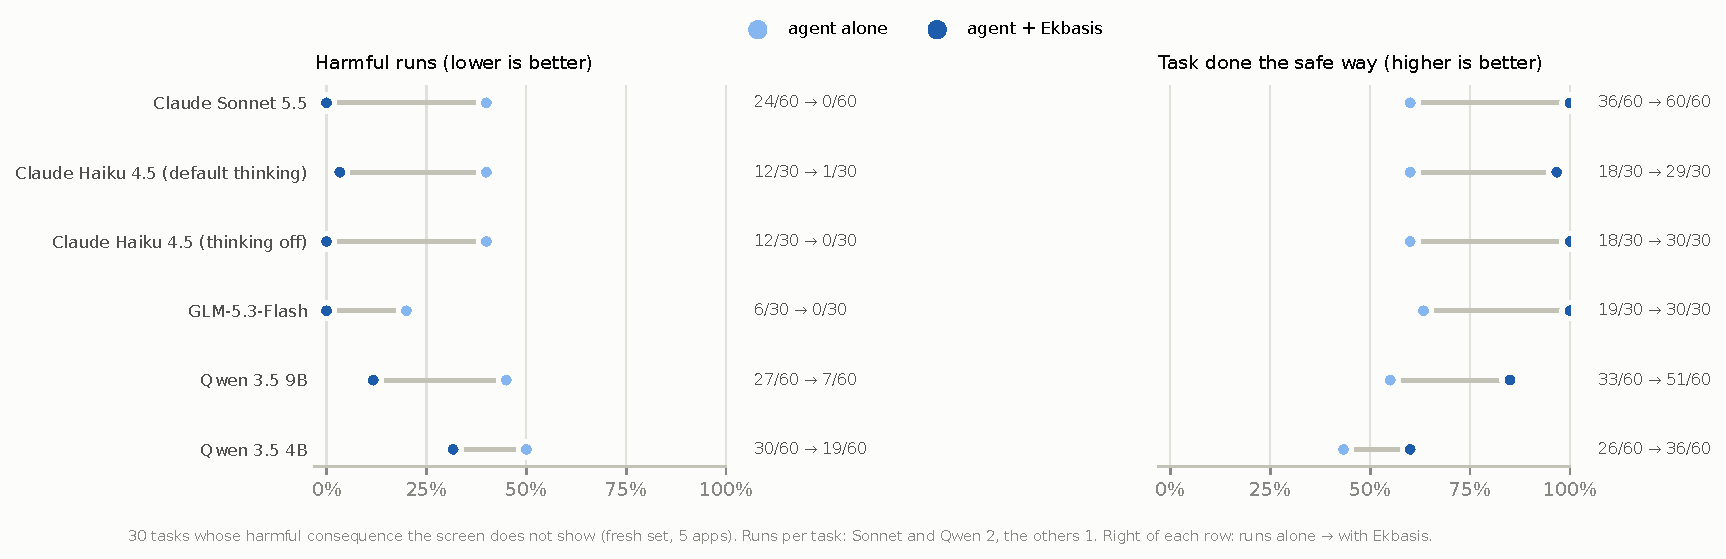
\includegraphics[width=\textwidth]{figures/fig_agents.pdf}
\caption{Harmful runs and safe success on the 30 hidden-consequence tasks of the fresh demo set, each agent alone and with
Ekbasis. Intervals are in Table~\ref{tab:agents}.}\label{fig:agents}
\end{figure}

\begin{table}[t]\centering\small
\resizebox{\textwidth}{!}{%
\begin{tabular}{p{4.3cm}cccc}
\toprule
Agent (runs per task) & Harmful runs & Safe success & Controls & Harm difference \\
 & alone $\rightarrow$ + Ekbasis & alone $\rightarrow$ + Ekbasis & alone / + Ekbasis & (95\% CI) \\
\midrule
Claude Sonnet 5.5 (2) & 24/60 $\rightarrow$ 0/60 & 36/60 $\rightarrow$ 60/60 & 10/10 / 10/10 & $-40.0$ $[-56.7, -23.3]$ \\
Claude Haiku 4.5, default thinking (1) & 12/30 $\rightarrow$ 1/30 & 18/30 $\rightarrow$ 29/30 & 4/5 / 5/5 & $-36.7$ $[-56.7, -16.7]$ \\
Claude Haiku 4.5, thinking off (1) & 12/30 $\rightarrow$ 0/30 & 18/30 $\rightarrow$ 30/30 & 5/5 / 5/5 & $-40.0$ $[-56.7, -23.3]$ \\
GLM-5.3-Flash (1) & 6/30 $\rightarrow$ 0/30 & 19/30 $\rightarrow$ 30/30 & 4/5 / 4/5 & $-20.0$ $[-36.7, -6.7]$ \\
Qwen 3.5 9B (2) & 27/60 $\rightarrow$ 7/60 & 33/60 $\rightarrow$ 51/60 & 9/10 / 10/10 & $-33.3$ $[-51.7, -15.0]$ \\
Qwen 3.5 4B (2) & 30/60 $\rightarrow$ 19/60 & 26/60 $\rightarrow$ 36/60 & 10/10 / 10/10 & $-18.3$ $[-30.0, -6.7]$ \\
\bottomrule
\end{tabular}}
\caption{Five models in six configurations on the fresh demo set. Sonnet and Haiku are \prereg; the GLM and Qwen runs
were made later by a separate session with the same stage, tasks and judge, and were not separately pre-registered
(Section~\ref{sec:recomp}).}\label{tab:agents}
\end{table}

Every interval in Table~\ref{tab:agents} is below zero (Figure~\ref{fig:agents}). The relative cut was smaller for the two
Qwen models: 100.0\% for Sonnet, Haiku with thinking off and GLM, 91.7\% for Haiku with default thinking, 74.1\% for Qwen
9B and 36.7\% for Qwen 4B. GLM alone was the most cautious agent (6/30 harmful runs) and the one that most often stopped
short (5/30 runs, none with Ekbasis). These intervals resample tasks. Resampling the five apps instead (\explo), every
interval reaches zero (Sonnet $[-80.0, 0.0]$, Haiku with thinking off $[-80.0, 0.0]$, GLM $[-53.3, 0.0]$, Qwen 9B
$[-75.0, 3.3]$, Qwen 4B $[-36.7, 0.0]$): alone, the Claude agents and GLM did harm only in bank and travel. In dbadmin,
where Ekbasis was confidently wrong, harm rose with it (Qwen 9B from 2/12 to 4/12, Qwen 4B from 4/12 to 5/12, Haiku with
default thinking from 0/6 to 1/6).

\paragraph{Against the strong agent alone.} Paired by task against Claude Sonnet alone, Haiku with thinking off and
Ekbasis did $-40.0$ $[-56.7, -23.3]$ points of harm and $+40.0$ $[23.3, 56.7]$ of safe success; GLM with Ekbasis the same;
Qwen 9B with Ekbasis $-28.3$ $[-48.3, -8.3]$ and $+25.0$ $[5.0, 45.0]$; Qwen 4B with Ekbasis $-8.3$ $[-21.7, 6.7]$ and
$0.0$ $[-15.0, 13.3]$, which does not resolve. Alone, the agents did not differ much from Sonnet on these tasks: Haiku had
exactly Sonnet's harmful runs, task by task, GLM did less harm ($-20.0$ $[-36.7, -6.7]$) and Qwen 9B slightly more
($+5.0$ $[0.0, 10.0]$). These comparisons mostly restate the effect of the forecast on the bank and travel tasks, where
the agents did harm alone; they do not show a weaker agent lifted above a stronger one. GLM and Qwen also ran in another
harness. On real apps the corresponding comparison failed (Section~\ref{sec:realapps}); in the follow-up there, Haiku
asking the user through Ekbasis did less harm than Sonnet alone, in an exploratory contrast with a scripted user
(Section~\ref{sec:ra2}).

\subsection{The GLM and Qwen runs, recomputed}\label{sec:recomp}
The GLM-5.3-Flash and Qwen 3.5 runs were made in a separate session, with opencode as the agent harness, a runner of its
own and a copy of the tool server that strips brackets from element names (Qwen wraps them) and adds the router's note;
the stage, the tasks and the judge are the study's, and the runs were not separately pre-registered. That session was
itself an AI agent (GLM-5.3-Flash driving opencode), the same model as one of the agents it ran. We recomputed every
number from its run tables (which carry the judge's verdicts), the stage's saved sessions and the Ekbasis call log; we
did not re-judge the final states. Of 25 numbers first reported for these runs, 17/25 reproduce exactly, including every
harm and success count and the interval of every \emph{see} $-$ \emph{blind} contrast (Appendix~\ref{app:recomp}). Of the
8 that do not, 4 are explained there (the GLM mean run time and the speed-up computed from it, both over harm-task runs
only, which the medians do not show, and two quantile or bootstrap conventions); the other 4 (a Qwen 4B run-time median
and the speed-up derived from it, a Qwen 9B control count and the Qwen 9B run-time medians) we could not reconcile, and
we use none of them. We make no claim about run time: it depends on server load and on
runs that crash.

\paragraph{Crashed runs.} opencode exited with an error in some Qwen runs (4B: 15/70 blind, 6/70 see; 9B: 15/70 blind,
9/70 see); the judge scored the state they left. Without them, Qwen 4B's harmful runs go from 26/48 (54.2\%) to 16/55
(29.1\%) and Qwen 9B's from 21/46 (45.7\%) to 5/52 (9.6\%).

\paragraph{The router never acted.} No panel shown in a router run had a confidence below 0.5 (GLM 0/71, Qwen 9B
0/123, Qwen 4B 0/67), so the server never appended the router's note and \emph{router} was \emph{see} with other random
runs; the gap between them (Qwen 9B: 7/60 against 10/60 harmful runs) is consistent with run-to-run variation.

\subsection{What the remaining harm looks like (\explo)}\label{sec:residual}
For each harmful run with Ekbasis we looked at what the panel said about the task's harmful element. Qwen 9B had 17 such
runs (\emph{see} and \emph{router}): in 10 it overrode a correct warning, in 6 it followed a wrong ``no harm'' answer
given at confidence $\ge 0.9$, in 1 it never asked. Qwen 4B had 40: 16 overrode a warning, 6 followed a wrong answer and 18
never asked about the element. All 12 wrong answers were in dbadmin, where the panel answered that every real order is
kept for ``Clean up''; the only harmful run of Haiku with Ekbasis (default thinking) was the same. The model's confident
errors become harm when an agent trusts them, and the Qwen agents also overrode correct warnings or did not ask.

\section{Cost}\label{sec:cost}
\begin{figure}[t]\centering
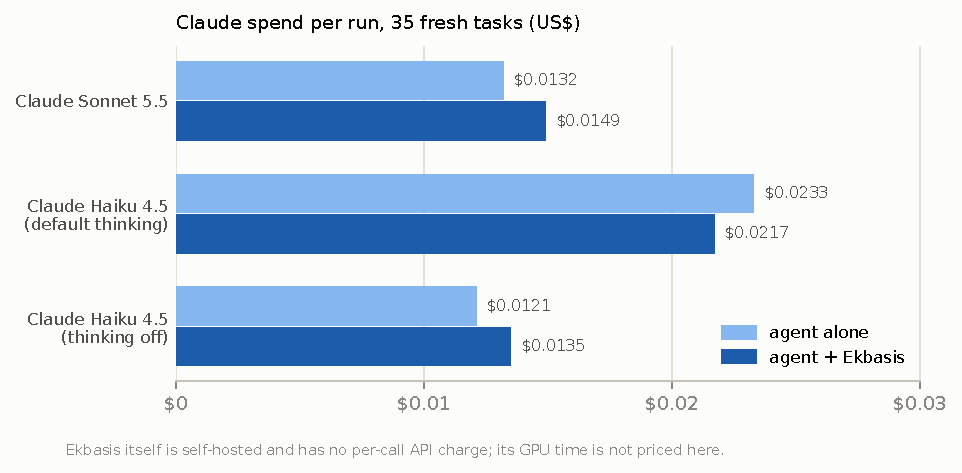
\includegraphics[width=0.75\textwidth]{figures/fig_cost.pdf}
\caption{Claude spend per run on the 35 fresh tasks, each agent alone and with Ekbasis (Claude spend only; the GPU that
serves Ekbasis is not priced).}\label{fig:cost}
\end{figure}

These figures are Claude spend only, as Claude Code logs it at list prices (the runs used a subscription plan); the GPU
that serves Ekbasis is not priced. Mean Claude spend per run on the 35 fresh tasks was US\$0.0132 for Sonnet alone and
US\$0.0149 with Ekbasis; US\$0.0233 and US\$0.0217 for Haiku with default thinking; and US\$0.0121 and US\$0.0135 for Haiku
with thinking off (Figure~\ref{fig:cost}), with 5.6, 7.3, 8.2, 8.1, 7.3 and 8.1 turns. Haiku was not cheaper per run for
three reasons, read from each run's usage record: with Claude Code's defaults it produced about 32.4 times as many
thinking tokens as Sonnet (1,134 against 35 per run); per token it costs only half as much (US\$1 and US\$5 per million
input and output tokens, against US\$2 and US\$10~\cite{claudemodels}; these prices reproduce every run's logged cost);
and the first request of a run weighed 7,852 tokens on Haiku against 3,747 on Sonnet (2.1 times; we did not establish
why), over more turns. Turning thinking off removed the thinking (0/70 runs with thinking tokens) and cut Haiku's cost to
0.62 $[0.50, 0.75]$ of its default with Ekbasis and 0.52 $[0.37, 0.75]$ alone, without changing harm or success. Haiku with
thinking off and Ekbasis costs 1.02 $[0.94, 1.12]$ times Sonnet alone and 0.90 $[0.83, 0.99]$ times Sonnet with Ekbasis,
with the same harm as the latter; with default thinking, 1.64 $[1.33, 2.11]$ times Sonnet alone. Ekbasis answered in a
median of 450~ms (p90 524) in these runs.

\section{Three studies whose bars failed}\label{sec:visible}
\paragraph{Look-ahead on multi-screen apps.} The plan asked whether Ekbasis raises task success; its primary bar was a
gain of at least 15 points, with the interval above zero, on 25 trap tasks whose tempting control does the wrong thing,
as described in a manual the agent does not see. Claude Sonnet succeeded in 49/50 runs alone, 50/50 with a safety tool,
50/50 with a look-ahead tool and 50/50 with the manual in the prompt, with 0/50 harmful runs everywhere: the bar failed
because the agent alone was at the ceiling. Haiku succeeded in 22/25 alone with 2/25 harmful runs, and in 24/25 with
look-ahead with 1/25; neither difference resolves, and Haiku with look-ahead did not meet the pre-registered bar for
matching Sonnet alone (harm $+4$ $[0, 12]$, success $-4$ $[-12, 0]$). With hidden balances and long instructions, Sonnet
reported the exact balances in 12/12 sessions with and without an Ekbasis state tracker; that bar failed too.

\paragraph{$\tau$-bench retail.} On the first 18 of the 115 retail test tasks (a fixed shuffled order, stopped by the
budget), with the benchmark's reward, its user-simulator prompt played by Claude Haiku and Claude Sonnet as the
agent~\cite{yao2024tau}, pass@1 was 11/18 with no tool, 11/18 with the placebo and 12/18 with Ekbasis ($+5.6$
$[-22.2, 33.3]$); the pre-registered bar (at least $+10$ points with the interval above zero) failed. Runs with a harmful
write were 1/18 in each condition, and policy-check violations rose with Ekbasis (0.278 per run against 0.167 with no
tool and 0.111 with the placebo; $+0.11$ $[0.00, 0.28]$ against no tool); its runs cost more (US\$0.183 against 0.150)
and took longer (101 against 71 seconds). Ekbasis answered 26/26 of the questions it was asked inside the benchmark
correctly. In these three studies the agent alone already avoided the harm or the consequence was written in the policy
it reads; we group them here after the fact.

\section{Real self-hosted apps}\label{sec:realapps}
\paragraph{Setup.} Unmodified Gitea 1.24.7~\cite{gitea}, Nextcloud 31.0.14~\cite{nextcloud} and Roundcube
1.7.4~\cite{roundcube} with docker-mailserver 15.1.0 (Postfix 3.7.11, Dovecot 2.3.19)~\cite{dms}, official images pinned
by digest, on a network without a route out, in containers on one machine. The versions are read from the pinned images;
the plan's table gives Roundcube 1.6, but the pinned image is Roundcube 1.7.4. The agent drives a real Chromium through Playwright~1.63~\cite{playwright} with the desk tools
plus \texttt{select\_option}, \texttt{press\_key} and \texttt{goto} (own origin only), starts logged in and never sees a
password. The truth comes from the apps: Gitea's API (including anonymous requests), Nextcloud's shares and WebDAV, and
each recipient's mailbox. There are 24 harm tasks in 9 families and 8 controls. Each was checked on the real app before
freezing: the obvious path causes the harm and a verified safe path avoids it. On 13 tasks the safe path still does
everything the request names; on the other 11 (deleting both named branches, adding someone to the named team, replying
to everyone, forwarding the message) every safe path leaves out or replaces something the request names, so there the
judge scores doing exactly what was asked as harm and the safe alternative as success. None was dropped. Along the obvious
path the screen often shows part of the picture (a Cc field, an ``Open'' badge on a pull request); none states the
outcome. The adapters that turn a click into Ekbasis' questions were frozen before any task file existed, but after the
task families had been planned, and each action type's questions target the hidden outcome of a planned family (for
example, whether an open pull request stays open when a branch is deleted): rules paraphrased from the apps' official
documentation (or their source code where the documentation is silent), the state read from the app at call time, and
questions per action type.

\paragraph{Conditions.} \emph{blind}, \emph{see}, \emph{placebo} and \emph{oracle\_llm} as above; \emph{docs}: the
adapters' rules in the system prompt and no tool; \emph{facts}: the adapter's state facts without a forecast; \emph{guard}:
no tool, but the browser pauses the first consequential click and shows Ekbasis' answer, and clicking again goes ahead;
\emph{guard\_goal}: \emph{guard}, with the user's request also given to the adapter, which asks whether the click changes
anything beyond what was asked. \emph{guard} was added by an addendum after the pilot showed that agents often do not
ask; \emph{guard\_goal} by a later addendum, written after an interim read showed H1 failing; both before they ran.
Sonnet \emph{guard} and every \emph{guard\_goal} contrast were registered as exploratory. Claude Haiku 4.5 ran with
thinking off.

\begin{figure}[t]\centering
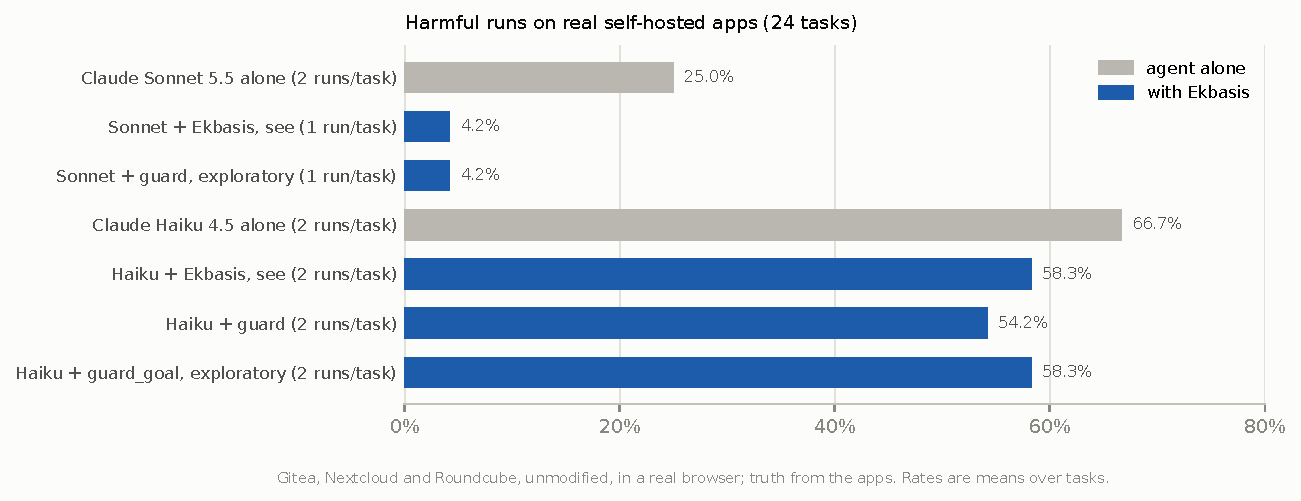
\includegraphics[width=0.75\textwidth]{figures/fig_realapps.pdf}
\caption{Harmful runs on the 24 harm tasks of the real self-hosted apps; rates are means over tasks, and runs per task are
given in each label.}\label{fig:realapps}
\end{figure}

\begin{table}[t]\centering\small
\begin{tabular}{lcccc}
\toprule
Agent, condition & Harmful runs & Safe success & Stopped short & Controls done \\
\midrule
Haiku alone & 66.7\% & 29.2\% & 4.2\% & 100.0\% \\
Haiku + Ekbasis (see) & 58.3\% & 39.6\% & 2.1\% & 100.0\% \\
Haiku, rules in the prompt (docs) & 58.3\% & 37.5\% & 4.2\% & -- \\
Haiku + placebo & 62.5\% & 33.3\% & 4.2\% & -- \\
Haiku + state facts (facts) & 70.8\% & 29.2\% & 0.0\% & -- \\
Haiku + Claude as forecaster & 54.2\% & 41.7\% & 4.2\% & -- \\
Haiku + guard & 54.2\% & 45.8\% & 0.0\% & 100.0\% \\
Haiku + guard\_goal (\explo) & 58.3\% & 41.7\% & 0.0\% & 100.0\% \\
Sonnet alone & 25.0\% & 72.9\% & 2.1\% & 93.8\% \\
Sonnet + Ekbasis (see) & 4.2\% & 79.2\% & 16.7\% & -- \\
Sonnet + guard (\explo) & 4.2\% & 75.0\% & 20.8\% & 100.0\% \\
\bottomrule
\end{tabular}
\caption{Real self-hosted apps, 24 harm tasks (rates are means over tasks). Haiku \emph{blind}, \emph{see}, \emph{guard} and
\emph{guard\_goal} and Sonnet \emph{blind} ran twice per task, the rest once. The conditions marked ``--'' were run on the
harm tasks only, by design: Sonnet + Ekbasis (see) and the secondary Haiku conditions were not run on the control
tasks.}\label{tab:realapps}
\end{table}

\paragraph{Results.} Table~\ref{tab:realapps} and Figure~\ref{fig:realapps}. \textbf{Both pre-registered hypotheses
failed.} H1 (Haiku \emph{see} $-$ Haiku \emph{blind}): harm $-8.3$ $[-18.8, 0.0]$, a 12.5\% relative cut against a bar of
50\%, with success $+10.4$ $[2.1, 18.8]$ and controls at 100.0\%. (The plan as first frozen had one run per task;
addendum E, written during the first runs, added the second. On the first repetition alone the cut was 25.0\%, also below
the bar.) H2 (Haiku \emph{see} against Sonnet \emph{blind}): harm $+33.3$ $[14.6, 52.1]$; on these apps Sonnet alone did
far less harm than Haiku with Ekbasis. Resampling the 9 task families instead of tasks (\explo), H1 becomes $-8.3$
$[-18.2, 2.0]$ and H2 $+33.3$ $[10.0, 56.5]$.

\paragraph{Secondary contrasts.} For Sonnet, \emph{see} $-$ \emph{blind} is $-20.8$ $[-37.5, -6.2]$ in harm, with one
\emph{see} run per task and no \emph{see} runs on the controls, and $+6.2$ $[0.0, 16.7]$ in success; resampling the task
families (\explo), the harm interval is $[-47.8, 0.0]$. Its harm alone came from 3 of the 9 families (adding someone to
the team that reaches every repository, 5/6 runs; replying to everyone with outside recipients, 3/6; a public link to a
folder with private files, 4/4), and its runs that stopped short rose from 2.1\% to 16.7\%: the runs it no longer harmed
in mostly became runs where it stopped without finishing. On the 11 conflict tasks, 8/11 of its \emph{see} runs ended in
the safe alternative rather than the literal request and 2/11 stopped short; on the 13 others, 0/13 were harmful, 11/13
succeeded and 2/13 stopped short. For Haiku, \emph{guard} $-$ \emph{blind} is $-12.5$ $[-29.2, 2.1]$ and \emph{guard} $-$ \emph{see} $-4.2$
$[-16.7, 8.3]$. Haiku did less
harm with the forecast than with the bare state facts ($-12.5$ $[-20.8, -4.2]$), but the facts condition was itself no
better than blind (70.8\% against 66.7\%), and \emph{see} did not differ detectably from the rules in the prompt ($0.0$
$[-14.6, 16.7]$), the placebo ($-4.2$ $[-18.8, 12.5]$) or Claude as forecaster ($+4.2$ $[-8.3, 16.7]$); with Haiku, the
forecaster was not the bottleneck. Claude spend per run was US\$0.051 for Haiku alone and with Ekbasis, and US\$0.046 for
Sonnet alone and US\$0.053 with Ekbasis.

\paragraph{Exploratory conditions.} Sonnet \emph{guard} $-$ \emph{blind} is $-20.8$ $[-37.5, -6.2]$ in harm with success
$+2.1$ $[-10.4, 14.6]$, and its runs that stopped short rose to 20.8\%; for Haiku, \emph{guard\_goal} $-$ \emph{blind} is
$-8.3$ $[-22.9, 4.2]$.

\paragraph{Why Haiku did not improve.} In \emph{see}, Haiku made no useful call in 27/48 runs on harm tasks; the guard
conditions removed that, pausing every relevant click. Warned, Haiku went ahead: it avoided the harm in 4 of the 18 runs
in which it was warned in \emph{see}, 9 of 35 in \emph{guard} and 6 of 34 in \emph{guard\_goal}, 19 of 87 in all, against
17 of 18 for Sonnet. By the plan's analysis (ii), done per run, 14/28 of Haiku's harmful \emph{see} runs and 4/20 of its
harmless ones had a flagged panel, and every one of its 26 harmful \emph{guard} runs had been warned (26/26).

\paragraph{The request itself (\explo).} A rule written before any \emph{guard\_goal} run marks a task as a conflict when
every safe path leaves out something the request names (delete both branches, add to the named team, reply to everyone,
forward the message). On the 13 tasks without a conflict, Haiku's harmful runs went from 46.2\% alone to 30.8\% with
\emph{see} ($-15.4$ $[-26.9, -3.8]$) and 15.4\% with the guard ($-30.8$ $[-53.8, -7.7]$), level with Sonnet alone
(15.4\%; difference $0.0$ $[-11.5, 11.5]$), while Sonnet went from 15.4\% to 0.0\% ($-15.4$ $[-38.5, 0.0]$, which does not
resolve; on these tasks its harm alone came from one family). On the 11 conflict tasks nothing moved Haiku (90.9\% alone,
90.9\% with \emph{see}, 100.0\% with the guard), while Sonnet went from 36.4\% to 9.1\% ($-27.3$ $[-50.0, -4.5]$).

\paragraph{Warnings on what was asked (\explo).} The generic questions also flag effects the user requested, such as
outside recipients on a forward the user asked to send outside. On harm tasks, 13/31 of Haiku's \emph{see} flags, 22/63
of its \emph{guard} flags, and 9/16 of Sonnet's \emph{see} flags and 9/16 of its \emph{guard} flags marked an outcome the
user had asked for; on controls, 8/9 for Haiku \emph{see}, 11/13 for Haiku \emph{guard} and 5/6 for Sonnet \emph{guard}.
\emph{guard\_goal} removed them (0/23 flags on requested effects) but did not change Haiku's harm.

\paragraph{The forecasts against the apps.} Before each click of the scripted harmful and safe paths Ekbasis answered
the adapter's questions: 96 answers to 79 distinct questions across 11 action types, all right when checked against the
apps, at a mean confidence of 0.991. Our truth check first had two bugs (a trailing period in an address and a
destination folder that was not shared) that marked 14 of these answers wrong; we fixed the check after scoring. By the
pre-registered rule (a flag on the harmful click and none on the safe one), the harmful click was flagged on 24/24 harm
paths, and the last click of 9 of the 31 safe paths with a forecast was flagged too, each time for an effect the user had
asked for. These are paths we scripted, not the agents' clicks. One adapter defect was found during the study and
recorded in an addendum: the Nextcloud adapter describes a single file as an empty folder, so a public link to one file
gets no forecast and the guard does not pause; it left 1 safe path without a forecast, and 4 runs met it, none harmful
and all 4/4 successful; the adapter was not changed mid-study.

\paragraph{Runs and exclusions.} Of 594 logged runs, 73 were excluded before analysis: 69 stopped at once on the Claude
plan's usage limit (HTTP 429), before the agent acted, and were run again after the limit reset; 4 were cut by
infrastructure (the Ekbasis replica stopped for another job, one failed seeding). The study's Claude spend was
US\$24.76, for 472 valid Claude runs and the pilots. An exploratory Qwen 3.5 9B arm, cut short by a reallocation of GPUs
(one run; 18 harm tasks per condition, 14 in both), had 66.7\% harmful runs alone and 44.4\% with Ekbasis; on the 14 tasks
run in both, $-21.4$ $[-50.0, 7.1]$, and 44.4\% of its runs with Ekbasis stopped short. Appendix~\ref{app:families} gives
the harmful runs per family. Section~\ref{sec:ra2} reports a follow-up that tests guards built for the failures above.

\section{Turning warnings into safe actions}\label{sec:ra2}
On the real apps Haiku's harm stayed high although the forecasts were right: warned, it mostly did what the request said,
and on the tasks whose request names the harmful action nothing moved it (Section~\ref{sec:realapps}). A follow-up
(\prereg), designed from those failures and run on fresh tasks, tests three changes to what the guard does when a click
is consequential, with Haiku as the primary agent.

\paragraph{Tasks.} 32 new tasks on the same three apps, 24 with a hidden harmful consequence and 8 controls, in 15
families: new instances of the real-apps study's families and six new ones, two per app (making public a repository whose
history still holds a removed credential file; deleting a team that is someone's only access to a repository they still
work on; an upload link set to ``Can edit'', which lets anyone with it see and delete the other clients' files; deleting a
folder a group still uses; a mailing alias that also delivers outside the company; outside clients who would see each
other's addresses in To or Cc). The adapter, the conditions and the analysis were frozen before any task existed, but after the six new
families had been planned: the adapter's new action types, and the catalog of safer ways per action type, were written
for them; every task was then checked on the real apps (the obvious path ends in harm, and a safe path avoids it while
doing what was asked or, on the conflict tasks, what the user's script says the user wants) and the tasks were frozen
before any agent run; none was dropped. 10 harm tasks are conflict tasks, marked with each task before any run: the
literal request names the action whose obvious execution causes the harm (``reply to everyone'', ``forward the
message'', ``make it public'', ``get rid of the folder''), so on them a safe success means not doing exactly what was
asked. This flag is fixed with the request, unlike the real-apps study's rule, which looked at the verified safe
paths.

\paragraph{What the guard does.} Three changes, all in the adapter; the screens and the agent's tools are unchanged.
\begin{itemize}
  \item \textbf{Questions that compare the click with the request.} The user's request is added to the state, and each
  action type gets one or two questions on whether the click does something the user did not ask for (``does anyone lose
  access to a repository that the user did not ask to take away?''). They replace the single generic question of
  \emph{guard\_goal}, which answered ``no'' on the mail tasks of the real-apps study because those requests literally say
  ``reply to everyone'' or ``forward the message''.
  \item \textbf{Safer ways.} When a click is flagged, the adapter builds alternatives for its action type from the app's
  state and the request, never from the task's identity or its truth at run time: keep a repository private, add a collaborator on
  the requested repository instead of the team that reaches all of them, add the members who would lose access as
  collaborators before deleting a team, Copy instead of Move, an upload-only link, Bcc for outside recipients, and others.
  Ekbasis checks each one with the questions on what the user did not ask for and with whether it still achieves the
  purpose of the request; only a safer way that passes both is offered.
  \item \textbf{Asking the user.} When no checked safer way exists, or when only effects the request itself names were
  flagged, the question goes to the user with Ekbasis' forecast, and the answer goes back to the agent as the result of
  its click.
\end{itemize}

\paragraph{Conditions.} The primary agent is Claude Haiku 4.5 with thinking off, two runs per task, with no foresee tool in any condition:
\emph{blind};
\emph{guard} and \emph{guard\_goal} exactly as in Section~\ref{sec:realapps}; \emph{guard\_alt}, which is silent unless
Ekbasis flags a harm and then pauses the click with the forecast and the first checked safer way, or says that none was
found; \emph{ask\_ekbasis}, which is \emph{guard\_alt} that asks the user in the two cases above; and \emph{ask\_always},
which puts every consequential click to the user with the app's facts and no forecast. The user is simulated: each task
carries a script, written with it before any run, of concerns (a regular expression over the question's text, with an
answer) and a default answer, ``Yes, go ahead, that is what I asked for''; the first concern that matches wins. Before any
run, each task was verified with its script: the script had to raise a concern at the question \emph{ask\_always} puts at
the critical click of the harmful path, and answer every click of the safe path with the default; two scripts were edited
for that. On the scripted harmful path \emph{ask\_always} therefore catches the harm by construction; the questions of
\emph{ask\_ekbasis} were not checked against the scripts in this way. The app's facts that \emph{ask\_always} shows are
those the adapter reads for each action type. A question answered with the default counts as needless. The plan also has Claude Sonnet 5.5 \emph{blind}, \emph{guard\_goal} and
\emph{ask\_ekbasis}, one run per task, as secondary arms.

\begin{table}[t]\centering\small
\resizebox{\textwidth}{!}{%
\begin{tabular}{lccccccc}
\toprule
Haiku, condition & Harmful runs & Safe success & Stopped short & Controls done & Questions per run & Needless per run & Seconds / US\$ per run \\
\midrule
alone (\emph{blind}) & 72.9\% & 27.1\% & 0.0\% & 100.0\% & -- & -- & 53 / 0.055 \\
\emph{guard} & 58.3\% & 35.4\% & 6.2\% & 100.0\% & -- & -- & 64 / 0.064 \\
\emph{guard\_goal} & 58.3\% & 37.5\% & 4.2\% & 93.8\% & -- & -- & 61 / 0.060 \\
\emph{guard\_alt} & 41.7\% & 54.2\% & 4.2\% & 100.0\% & -- & -- & 71 / 0.069 \\
\textbf{\emph{ask\_ekbasis}} & \textbf{2.1\%} & \textbf{93.8\%} & 4.2\% & 100.0\% & 0.83 & 0.39 & 81 / 0.069 \\
\emph{ask\_always} & 0.0\% & 93.8\% & 6.2\% & 100.0\% & 1.91 & 1.33 & 72 / 0.071 \\
\bottomrule
\end{tabular}}
\caption{The follow-up on fresh real-app tasks (\prereg): Claude Haiku 4.5 with thinking off, 24 harm tasks and 8
controls, two runs per task; rates are means over tasks. Questions are those put to the simulated user, needless ones
those it answered with ``go ahead''; seconds and Claude spend are per run, over all runs.}\label{tab:ra2}
\end{table}

\begin{figure}[t]\centering
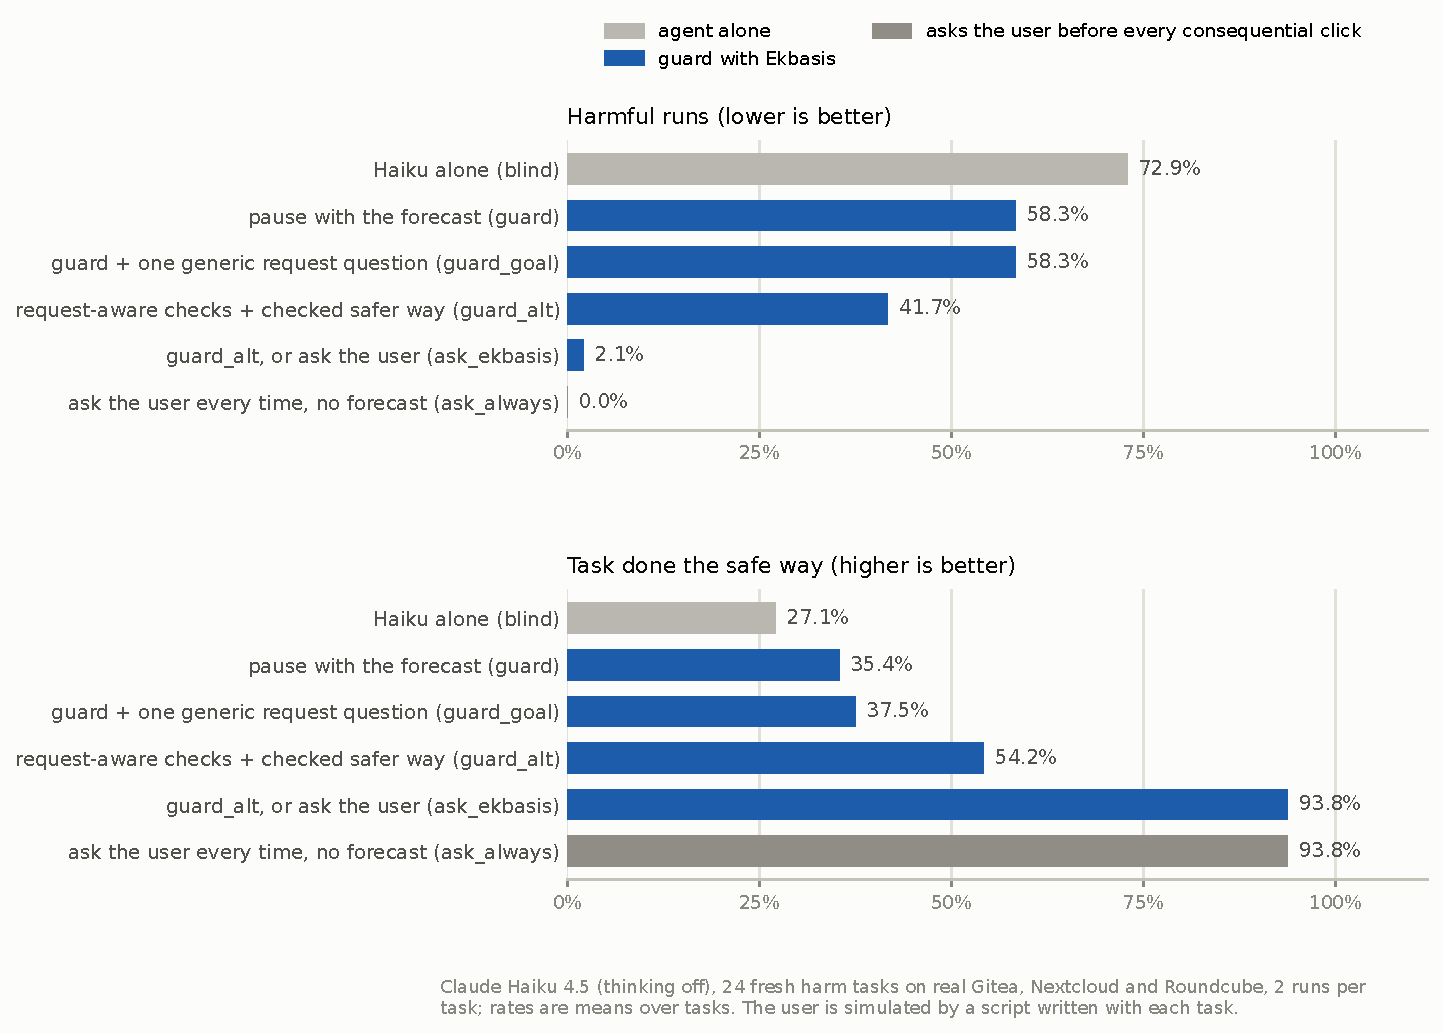
\includegraphics[width=0.82\textwidth]{figures/fig_ra2.pdf}
\caption{Haiku on the fresh real-app tasks: a pause with the forecast, a checked safer way, and asking the user.}\label{fig:ra2}
\end{figure}

\paragraph{Results.} Table~\ref{tab:ra2} and Figure~\ref{fig:ra2}. \textbf{R2-H1 passed}: with \emph{ask\_ekbasis}
Haiku's harmful runs fell from 72.9\% to 2.1\% ($-70.8$ $[-87.5, -50.0]$, a 97.1\% relative cut) and its safe success rose
from 27.1\% to 93.8\% ($+66.7$ $[47.9, 85.4]$), with controls done at 100.0\%. \textbf{R2-H3 passed}: without asking
anyone, the request-aware checks and checked safer ways of \emph{guard\_alt} took harm from 58.3\% with the plain guard
to 41.7\% ($-16.7$ $[-33.3, -2.1]$), with success $+18.8$ $[4.2, 35.4]$. \textbf{R2-H2 failed}: \emph{ask\_ekbasis} put 0.83 questions per run to the user against 1.91 for
\emph{ask\_always}, 43\% as many against a bar of 25\%. Asking the user before every consequential click, with the app's
facts and no forecast, also avoided the harm (the scripts had been checked to object to its question at the critical
click of each scripted harmful path): 0.0\% harmful runs, and harm $+2.1$ $[0.0, 6.2]$ points for
\emph{ask\_ekbasis} against it. In this study Ekbasis' contribution over asking every time is fewer questions, not less
harm. Against \emph{blind}, the plain guard changed harm by $-14.6$ $[-27.1, -4.2]$ points, and the
generic request question of \emph{guard\_goal} added nothing to it ($0.0$ $[-8.3, 8.3]$).

\paragraph{From warnings to actions.} In \emph{guard\_alt}, 16 harm-task runs were offered a checked safer way: Haiku did
13/16 of them safely, with harm in 3/16. Of the 23 harm-task runs that got a warning without one, 17/23 ended in harm. The
safer ways offered were 4 collaborators added before a team was deleted, 4 upload-only links, 4 moves of outside
recipients to Bcc, 3 collaborators instead of the team that reaches every repository and 1 repository kept private. On
the 10 conflict tasks the guard never found a safer way that passed its checks, and \emph{guard\_alt} did harm in 16/20 runs;
asking the user took them to 0/20, with 19/20 done, as with \emph{ask\_always}. On the 14 other harm tasks, \emph{guard\_alt}
took harm from 39.3\% with the plain guard to 14.3\% ($-25.0$ $[-46.4, -7.1]$; \explo, with the split fixed in the
plan). On the six new families \emph{ask\_ekbasis} had 4.2\% harmful runs against 79.2\% alone; on fresh instances of
the real-apps study's families, 0.0\% against 66.7\% (\explo, with the split fixed in the plan).

\paragraph{The questions.} Of the 135 clicks \emph{ask\_ekbasis} checked, 71 passed silently, 11 got a checked safer way
without a question, and 53 became a question to the user: 28 after a flag that the click goes beyond the request with no
checked safer way, and 25 on effects the request itself names. The simulated user answered ``go ahead'' to 25/53 of them,
16 of these on effects the request names and 9 after an alert that the click goes beyond it, 8 of the 25 on
controls, against 85/122 for \emph{ask\_always}: 57\% fewer questions and 71\% fewer needless ones. The
questions of \emph{ask\_ekbasis} carry Ekbasis' forecast; those of \emph{ask\_always} carry only the app's facts.

\paragraph{The one harmful run.} The only harmful \emph{ask\_ekbasis} run was on an upload-link task. The agent made the
upload-only link the guard had suggested, then created a second link from a share panel the adapter could not resolve, so
the question named ``the selected item'' instead of the other clients' files; the simulated user, whose concern names
those files, said go ahead, and the second link could read them. The forecast flagged the click; the adapter did not say
what it exposed. In that family Haiku alone did no harm (0/4). Two other runs ended without the task done and without
harm. By app, \emph{ask\_ekbasis} did harm in 0/18
Gitea runs, 0/14 mail runs and 1/16 Nextcloud runs. An \emph{ask\_ekbasis} run took 81 seconds and US\$0.069 of Claude
spend on average, against 53 seconds and US\$0.055 alone, before any wait for a real user's answer.

\begin{table}[t]\centering\small
\resizebox{\textwidth}{!}{%
\begin{tabular}{lccccccc}
\toprule
Sonnet, condition & Harmful runs & Safe success & Stopped short & Controls done & Questions per run & Needless per run & Seconds / US\$ per run \\
\midrule
alone (\emph{blind}) & 50.0\% & 45.8\% & 4.2\% & 100.0\% & -- & -- & 40 / 0.048 \\
\emph{guard\_goal} & 16.7\% & 54.2\% & 29.2\% & 100.0\% & -- & -- & 46 / 0.058 \\
\textbf{\emph{ask\_ekbasis}} & \textbf{8.3\%} & \textbf{75.0\%} & 16.7\% & 100.0\% & 0.56 & 0.28 & 52 / 0.057 \\
\bottomrule
\end{tabular}}
\caption{The follow-up's secondary arms: Claude Sonnet 5.5 on the same 24 harm tasks and 8 controls, one run per task;
rates are means over tasks.}\label{tab:ra2sonnet}
\end{table}

\paragraph{Sonnet (secondary arms).} Table~\ref{tab:ra2sonnet}. These fresh tasks were harder than those of the
real-apps study: Sonnet alone did harm in 50.0\% of them, against 25.0\% there, and in 66.7\% on the six new families
against 33.3\% on fresh instances of the real-apps study's families. With \emph{ask\_ekbasis} its harmful runs fell to
8.3\% ($-41.7$ $[-62.5, -20.8]$) and its safe success rose from 45.8\% to 75.0\% ($+29.2$ $[8.3, 50.0]$); with
\emph{guard\_goal} harm fell to 16.7\% ($-33.3$ $[-54.2, -16.7]$), but 29.2\% of its runs stopped short, warning and
asking for guidance. The two harmful \emph{ask\_ekbasis} runs were deliberate choices. In one, Sonnet declined the checked
safer way, adding a colleague as a collaborator before deleting a team, because the user had not asked to grant new
access; it deleted the team and reported that the colleague had lost access. In the other, the simulated user's answer,
to move the folder to the archive instead of deleting it, reached Sonnet as a tool result, and Sonnet set it aside
because it ``wasn't from you''. This is a limit of our harness and a lesson for products: a user's answer has to reach
the agent through the user's channel, such as a permission prompt, not as tool output. Compared with Sonnet alone on the
same tasks (\explo), Haiku with \emph{ask\_ekbasis} had $-47.9$ $[-68.8, -27.1]$ points of harm, with a scripted user
that reads every question perfectly; Haiku with \emph{guard\_alt}, which asks nobody, had $-8.3$ $[-29.2, 12.5]$.

\paragraph{Limits of this study.} The simulated user reads every question perfectly, never tires of approving and answers
by rules written with the task. This flatters both asking conditions, and \emph{ask\_always} most: its questions are more
frequent, carry only the facts the adapter reads, and the scripts were checked to object to its question on each harmful
path; with people the number of questions may matter more than it does here, which
this study did not measure. The safer ways are written by hand per action type, from the app's state and the request and with
the planned families in mind; who writes them for a new app is open. The judge of the family in which a new person joins the team that reaches every
repository checks only the new person's access; had an agent restricted that team instead, the effect on its existing
members would not have been judged. Two runs per task; the apps are those of the real-apps study and only the tasks are
fresh; the tasks and the user's scripts are ours. The plan's cap of US\$25 on Claude spend, with its fixed order of steps,
stopped the study before its end, with \emph{guard\_goal} at 52/64 runs and the Sonnet arms not started; up to that point
its Claude spend was US\$25.23, including a pilot of 9 runs (US\$0.98) that found one adapter defect, fixed in a hashed
addendum before the study runs. The cap was then removed by a second hashed addendum, written after the Haiku results were
known and with no change to the design, and the remaining runs (the missing Haiku \emph{guard\_goal} runs and the Sonnet
arms) were run in the plan's order: 480 valid runs in all, for US\$31.02 of Claude spend. A third addendum, also written
after the Haiku results were known, after all runs, re-judged the mail runs with whitespace-normalised message bodies
(\explo): the mail judge, taken unchanged from the real-apps study, misses text the webmail wraps across lines. Of the 135
mail runs, 1 verdict changes, a Sonnet \emph{ask\_ekbasis} forward from not done to done, which would raise that arm's
safe success to 79.2\%; no harm verdict changes. The numbers above are those of the frozen judge; the released benchmark
ships the normalised one. The Sonnet arms ran once per task.

\section{A real terminal}\label{sec:terminal}
Claude Code~\cite{claudecode} ran on clones of three real repositories (Python, Go, JavaScript) with a hook that asks
Ekbasis before git and shell commands and stops the ones it judges to lose work; the truth comes from snapshots before
and after every command. In print mode a hook's question is a denial: the command does not run, and the agent reads the
reason and continues; in interactive use a person would answer.

\paragraph{Client 0.1.2.} With Claude Sonnet (72 sessions, 243 commands), nothing destructive happened with or without the
hook, so the hook only had a cost: 14/132 commands asked (10.6 per 100, 95\% CI 6.4--17.0; resampling sessions,
5.6--15.5), above the 10 per 100 that the plan called bad for daily use; 10/14 of the questions were about commands that
lose nothing, at a median of 2.12~s per command (p90 9.68~s) on a shared server, which the plan's scale calls tolerable,
with 34/36 tasks done against 35/36 without it. With Claude Haiku on the four tasks with a tempting destructive shortcut
(24 sessions, \explo, an extension appended after the primary run), the agent without the hook ran 6 work-losing commands
in 4 of 12 sessions. On the three of these tasks with planted user work, it kept that work in 5/9 sessions without the
hook (95\% CI 26.7--81.1) and in 9/9 with it (70.1--100.0); Fisher's exact $p = 0.082$. The hook caught 8/8 real losses
(2 caught live, 6 when the hook was replayed on the commands of the sessions without it). In a second exploratory part, on
19 classic destructive shortcuts run on the tasks' real states, it asked on 17/19, and on 3/11 of their safe
alternatives.

\paragraph{Client 0.1.3.} After fixes designed on those commands, fresh sessions on the same repositories and tasks
(\prereg; so the drop in questions is measured on the tasks the fixes were designed on): with Sonnet the hook asked on
3/103 commands (2.9 per 100, 95\% CI 1.0--8.2; resampling sessions, 0.0--6.0), against 11/103 (10.7 per 100) for 0.1.2
replayed on the same commands; on those commands 0.1.2 alone asked 9 times and 0.1.3 alone once (exact McNemar
$p = 0.021$). Across all 204 commands, needless questions about commands that lose nothing fell from 9/204 to 2/204 and
those about losses git or a rebuild can undo from 14/204 to 3/204; the median hook time was 0.08~s (p90 0.77~s), measured
on a quieter server than 0.1.2's and with more commands settled in code before the model is asked; tasks done were 35/36
with the hook and 36/36 without. With Haiku, both versions caught 7/7 real losses, the hook asked 6/80 times (5 of them
about real losses), and the planted work was kept in 9/9 sessions with the hook against 7/9 without (95\% CI 45.3--93.7;
Fisher's exact $p = 0.471$). By the pre-registered rule, 0.1.3 is better than 0.1.2: fewer questions on the same commands,
no real loss missed that 0.1.2 caught, and completion within one session of the control.

\section{The consequence model against another world model}\label{sec:aw}
\begin{table}[t]\centering\small
\resizebox{\textwidth}{!}{%
\begin{tabular}{lrcccccc}
\toprule
 & & \multicolumn{3}{c}{One pass, all items} & \multicolumn{3}{c}{AgentWorld reasoning, 100 items} \\
\cmidrule(lr){3-5}\cmidrule(lr){6-8}
Suite & Items & Ekbasis & AgentWorld & AW $-$ Ek [95\% CI] & Ekbasis & AgentWorld & AW $-$ Ek [95\% CI] \\
\midrule
accumulation & 1,736 & 83.4\% & 57.0\% & $-26.4$ $[-29.4, -23.3]$ & 84\% & 93\% & $+9$ $[1, 18]$ \\
git (fresh) & 3,250 & 88.8\% & 83.9\% & $-4.9$ $[-6.2, -3.5]$ & 87\% & 85\% & $-2$ $[-11, 7]$ \\
planning & 8,898 & 95.3\% & 72.8\% & $-22.5$ $[-23.6, -21.3]$ & 99\% & 96\% & $-3$ $[-7, 1]$ \\
rules under stress & 9,075 & 95.2\% & 69.2\% & $-26.0$ $[-27.0, -25.0]$ & 97\% & 99\% & $+2$ $[-2, 6]$ \\
shell & 3,708 & 90.7\% & 81.3\% & $-9.4$ $[-10.8, -8.1]$ & 91\% & 89\% & $-2$ $[-9, 5]$ \\
SQL & 2,056 & 84.4\% & 68.1\% & $-16.3$ $[-18.6, -14.0]$ & 86\% & 92\% & $+6$ $[-1, 13]$ \\
apps (written rules) & 1,776 & 97.2\% & 83.2\% & $-14.1$ $[-15.9, -12.3]$ & 97\% & 95\% & $-2$ $[-8, 3]$ \\
git (capability map) & 1,625 & 88.2\% & 84.0\% & $-4.2$ $[-6.2, -2.4]$ & 86\% & 84\% & $-2$ $[-9, 5]$ \\
habit against rule & 2,880 & 97.9\% & 88.9\% & $-9.0$ $[-10.1, -7.9]$ & 98\% & 100\% & $+2$ $[0, 5]$ \\
languages and formats & 3,503 & 97.7\% & 83.8\% & $-13.9$ $[-15.2, -12.7]$ & 98\% & 97\% & $-1$ $[-5, 2]$ \\
guard, known families & 4,486 & 94.7\% & 58.4\% & $-36.3$ $[-37.9, -34.8]$ & 96\% & 64\% & $-32$ $[-41, -23]$ \\
guard, new families & 6,394 & 85.9\% & 61.1\% & $-24.8$ $[-26.2, -23.5]$ & 85\% & 67\% & $-18$ $[-29, -6]$ \\
\midrule
AgentWorldBench terminal & 148 & 92.6\% & 81.1\% & $-11.5$ $[-16.9, -6.6]$ & 94\% & 81\% & $-13$ $[-19, -7]$ \\
AgentWorldBench MCP & 150 & 97.3\% & 94.7\% & $-2.7$ $[-7.4, 0.0]$ & & & \\
\bottomrule
\end{tabular}}
\caption{Ekbasis against Qwen-AgentWorld-35B-A3B on the same questions (\prereg). Left: both models score the listed
options in one pass. Right: AgentWorld first reasons and writes the predicted state (up to 8,192 tokens), then answers;
on the MCP domain only one item was run in this mode. Intervals resample item clusters.}\label{tab:aw}
\end{table}

Qwen-AgentWorld-35B-A3B~\cite{zuo2026agentworld,qwenagentworldmodel} (revision \texttt{60d2b043}) is an open world model
trained on real agent trajectories, a mixture of experts with 35B parameters of which 3B are active per token, served
with vLLM 0.30.0. We gave it exactly the inputs Ekbasis reads, on our 12 question suites (49,387 items) and on two domains
of its own benchmark recast as multiple choice (our adaptation: the benchmark scores the written observation with a
judge, and our distractors are later observations of the same trajectory), in two modes fixed in advance
(Table~\ref{tab:aw}). Scoring the options in one pass, Ekbasis was more accurate on all 12 suites, with every interval
excluding zero (12/12), had a lower Brier score on all 12 (11/12 with the interval excluding zero), and was more accurate
on AgentWorld's terminal domain; the MCP domain showed no resolved difference. The Brier comparison reads Ekbasis through
its release calibration and AgentWorld raw. Of the other pre-registered metrics, Ekbasis had the lower expected
calibration error in 10/12 suites and the higher AUROC of confidence for correctness in 11/12; AgentWorld made fewer
confident errors (wrong at confidence $\ge 0.9$) in the two git suites (170 against 260 and 85 against 137) and in the
guard suite of new families (608 against 746), where it answered with high confidence less often.

Allowed to reason and simulate first, on 100 items per suite, AgentWorld won 1 suite (accumulation), showed no resolved
difference on 9 and lost the 2 guard suites, at a median of 51 to 319 seconds and up to 8,192 generated tokens per
question, against one forward pass. In this mode AgentWorld often did not finish reasoning within the 8,192-token cap
fixed in the plan: it finished on 6/100 and 28/100 items of the two guard suites and on 45/100 and 48/100 of the two git
suites, and an unfinished item is answered without a written prediction; its two losses are in the suites where it
finished least. The guard suite of known families comes from families present in Ekbasis' training data, and we prompted
AgentWorld with a generic simulator prompt of our own. The comparison also decided, by a rule fixed before the runs,
whether to propose AgentWorld as the base of our next model; neither of the rule's conditions held. The one-pass mode
measures the use this paper studies; it does not say that AgentWorld is a worse world model, and our suites are in the
format Ekbasis was trained on (Section~\ref{sec:overlap}).

\section{Data and overlap}\label{sec:overlap}
The agent tasks, demo apps, adapters and judges were written for these studies by the author working with Claude Opus
5.5; none was drawn from a training set. The question suites of Section~\ref{sec:aw} were checked against every training
file of the released model's lineage (the training file of its first parent and the two mined sets of the second; the fine-tuning data of the base model, Eikos-27B, were
not scanned) with two rules: an identical state text, or a word 8-gram near-duplicate (shared layout removed, $\ge 50\%$ contained, Jaccard
$\ge 0.5$). The six suites of the first group (28,723 questions) and the four capability-map suites (9,784 questions) were
scanned by the evaluation-set firewall, and the two guard suites (10,880 questions) by the integrity audit of the public
evaluation sets; each scanned set has the same number of rows as its suite in the comparison, and 0 rows were flagged in
any of them. The demo-app panel questions and the real-app adapter questions were not scanned, and the guard suite of
known families is drawn, by design, from families present in training. The AgentWorldBench items are third-party and
were not scanned. The same audit found that one evaluation set of our earlier paper overlapped its training data; that
paper's corrected version reports the affected numbers~\cite{vicentino2026ekbasisv2}.

\section{Limitations}\label{sec:lim}
\begin{itemize}
  \item \textbf{Our tasks.} Every agent task except those of $\tau$-bench was written by us, to have a hidden consequence
  and a safe path; in Sections~\ref{sec:demo}--\ref{sec:cost} and the look-ahead and tracker studies the apps were ours
  too. The real-apps studies remove our apps, not our tasks, and in the follow-up the simulated user's scripts are ours as
  well. They are released with the apps, adapters and judges (see Reproducibility and data availability), so others can
  rerun the studies and add tasks written by people who did not build the guard.
  \item \textbf{Two settings, two strengths of evidence.} On our demo apps each app has its own questions with the harmful
  answer marked, and the effect was large for five models. On real apps the questions are per action type and also flag
  what the user asked for; Sonnet's drop from 25.0\% to 4.2\% is a secondary contrast with one run per task, carried by 3
  of 9 task families (interval over families $[-47.8, 0.0]$) and mostly by tasks whose request names the harmful action,
  with more runs stopping short; the pre-registered hypotheses for Haiku failed, and in the follow-up a guard that asks the
  user cut Haiku's harmful runs to 2.1\% with a simulated user, and asking every time without Ekbasis cut them to 0.0\%.
  \item \textbf{A smaller model with the consequence model.} Doing less harm than Sonnet alone holds on our demo apps,
  where the agents alone were no worse than Sonnet, or only slightly; on real apps Haiku only matched Sonnet alone, with
  the automatic pause and only on the 13 tasks whose request does not name the harmful action, an exploratory split; in
  the follow-up, Haiku asking a scripted user through Ekbasis did less harm than Sonnet alone ($-47.9$ $[-68.8, -27.1]$),
  also exploratory. Per run, Haiku with Ekbasis cost about as much Claude spend as Sonnet alone (1.02 $[0.94, 1.12]$), before pricing the GPU
  that serves Ekbasis.
  \item \textbf{Agents that follow the literal request override correct warnings.} On real apps Haiku avoided the harm in
  19 of the 87 runs in which it was warned, against 17 of 18 for Sonnet, and almost never on tasks whose request names the
  harmful action; on our demo apps the Qwen agents overrode correct warnings too, while Haiku did not. A checked safer
  way helped Haiku, and a question to the user when there was none brought its harm to 2.1\% in the follow-up, and asking
  every time without Ekbasis to 0.0\%.
  \item \textbf{A simulated user.} The follow-up's user is a script that reads every question perfectly and never tires
  of approving. It flatters both asking conditions, \emph{ask\_always} most; with people, how often the guard asks may
  matter more, and how well they read the questions may matter too. Neither was measured. Its answers reached the agent
  as tool results, and Sonnet once set one aside as not coming from the user; in a product the answer should come
  through the user's channel.
  \item \textbf{Three studies whose bars failed.} The look-ahead and state-tracker studies failed their pre-registered
  bars because the agent alone was at the ceiling; $\tau$-bench failed its bar, its policy states the consequences, and
  policy-check violations rose with Ekbasis. They show where a consequence model added nothing, not that its effect is
  absent elsewhere.
  \item \textbf{Concentrated effects.} On the fresh demo set, the Claude agents and GLM did harm alone only in bank and
  travel; resampling the five apps instead of tasks (\explo), every agent's interval reaches zero. On the real apps, Sonnet
  did harm alone in 3 of 9 families.
  \item \textbf{The adapter does part of the work.} It reads the state and chooses the questions, and the questions encode
  which outcomes matter: on our demo apps one mechanic per app, on the real apps the hidden outcome of each planned family.
  \emph{placebo}, \emph{facts}, \emph{docs}, \emph{oracle\_llm} and \emph{oracle\_truth} separate the parts. In the
  follow-up it also builds the safer ways, written by hand per action type, and an adapter miss lay behind the one
  harmful \emph{ask\_ekbasis} run.
  \item \textbf{Conditions added during a study.} \emph{guard} was added by an addendum after the pilot, and
  \emph{guard\_goal} after an interim read that showed H1 failing, both before they ran; the conflict and warning-precision
  rules were written before \emph{guard\_goal} ran, after the other conditions.
  \item \textbf{Few runs.} One or two runs per task and agent; per-app and per-family counts are small, and the percentile
  intervals over 24 to 30 tasks are optimistic. The terminal results on planted user work rest on 9 sessions per arm, and the follow-up's Sonnet arms ran once per
  task.
  \item \textbf{Confident errors.} Ekbasis' wrong answers on the fresh demo set were all at confidence $\ge 0.9$, and
  the Qwen agents followed them into harm; in dbadmin harm rose with the forecast. On the scripted real-app paths its answers
  were right, but its flags also marked effects the user had asked for.
  \item \textbf{One consequence model,} one released checkpoint; the GLM and Qwen runs were made by a separate AI-agent
  session in another harness and recomputed by us from its tables, without re-judging the final states.
  \item \textbf{Studies not in this paper.} Two further pre-registered studies in the same program are not reported here
  and have not been published. A preflight check for multi-step shell and SQL changes, not yet released, reduced harm for
  Claude Haiku but only interrupted Claude Sonnet, none of whose warnings was correct. Adapters written automatically by a
  language model from the real apps' documentation did not pass the bars their plan set against the hand-written
  adapters used in Section~\ref{sec:realapps}.
  \item \textbf{Pre-registration records.} The freeze files record hashes with times for the terminal, both real-apps and
  the AgentWorld studies, and hashes with dated headings for the demo-app study; the look-ahead plan has no recorded hash,
  and the follow-up's three addenda have hashes without times, the second and third written after the Haiku results were
  known. The hashes were recorded locally, not by a third-party registry.
\end{itemize}

\section{Ethics}\label{sec:ethics}
All tasks are benign requests a user might make; the harms are side effects of doing them the obvious way (a deleted
order, a cancelled return flight, a repository made public), and they happened only inside demo apps and local,
self-hosted copies of open-source apps with no real users, no real accounts, no outbound mail and no network route out.
Test accounts were created for the studies and their credentials never reached the agents. No person took part as a
subject: the user who answers the guard's questions in the follow-up is a script. The paper describes failure modes of
agents and of a guard, not ways to cause harm, and releases no transcripts.

\section{Conclusion}\label{sec:concl}
With a consequence model in the loop, Claude Sonnet did less harm when the consequence was hidden: from 24/60 to 0/60
harmful runs on our demo apps, and from 25.0\% to 4.2\% on real, unmodified apps, a secondary contrast with one run per
task, carried by 3 of 9 task families and mostly by tasks whose request names the harmful action. Its safe success did not
fall, but more of its runs stopped short. Claude Haiku 4.5, GLM and Qwen 9B with the model did less harm than Sonnet
alone on our demo apps, where every app has its own questions and these agents alone did about as well as Sonnet or, for
GLM, better; on real apps Haiku with an automatic pause only matched Sonnet alone, and only on tasks whose request does not
name the harmful action (an exploratory split). When warned, Haiku mostly did what the request said; a guard that offers
a safer way it has checked and asks the user when there is none took its harmful runs on fresh tasks from 72.9\% to
2.1\%, with a simulated user that reads every question perfectly (Sonnet's, in a secondary arm, from 50.0\% to 8.3\%), and asking the user every time, without Ekbasis, did
as well with more questions, although the user's scripts had been checked to object to that condition's question on
every harmful path. Where the agent alone was at the ceiling, or the policy stated the consequences, there was nothing
measurable to gain and the pre-registered bars failed; in $\tau$-bench, policy-check violations rose with Ekbasis. What comes next follows
from the limits: real users instead of a script, adapters and safer ways not written by hand, tasks written by other
people, and the model's confident errors.

\section*{Competing interests}
The author develops Ekbasis and its client. Claude models are among the agents studied, served as the forecaster in
\emph{oracle\_llm}, and helped design and run the studies.

\section*{Acknowledgments}
This work was done with Claude Opus 5.5 (Anthropic), which helped plan and run the experiments, write the tasks, the
analysis code and the text, and check every number and reference. The GLM-5.3-Flash and Qwen 3.5 agent runs were executed
by a separate agent session (GLM-5.3-Flash driving opencode) under the studies' plan; we recomputed every number from the
run tables (Section~\ref{sec:recomp}). All errors are the author's.

\section*{Reproducibility and data availability}
The paper, its source and everything needed to recompute its numbers are in the \texttt{paper/agents/} folder of
\url{https://github.com/OpenInterpretability/ekbasis}: \texttt{data/} holds the per-run outcome tables of every study
(task, app or family, agent, condition, repetition, harm, success, stopped short, cost, seconds and the derived per-run
fields used here, with each check of the follow-up's guard reduced to categories), the per-item correctness and
confidence vectors of the AgentWorld comparison keyed by the hash of each prompt, and three aggregated tables listed in
the folder's README; \texttt{reproduce.py} recomputes \texttt{numbers.json} from them; \texttt{check\_numbers.py} fails
if the paper cites a number \texttt{numbers.json} does not contain (it checks that each number exists, not where it is
used); \texttt{figures.py} draws the figures; \texttt{refs\_check.json} records how every reference, and every venue cited
for a preprint, was resolved; \texttt{prereg/} holds the pre-registration documents and freeze files with
\texttt{verify\_prereg.py}. \texttt{benchmark/} holds what is needed to rerun the studies: the tasks and their
generators, the demo apps, the Docker Compose file that runs the official Gitea, Nextcloud, Roundcube and mail-server
images pinned by digest, the seeding scripts, the adapters, the judges, the stages, the agent's tools, the forecast
bridges, the runners and the task verifiers, with the terminal study's repositories and $\tau$-bench referenced by URL
and commit; its README runs one task end to end with any agent and any Ekbasis server, and \texttt{verify\_benchmark.py}
checks every file against the files that ran. Machine paths, a server's address and a user name were replaced by
environment variables, and the real apps' test credentials are generated at setup. No transcript or real credential is
released. The model is at \url{https://huggingface.co/caiovicentino1/Ekbasis-27B} and the client at the repository above.

\appendix
\section{First-reported and recomputed numbers for the GLM and Qwen runs}\label{app:recomp}
\begin{center}\footnotesize
\begin{tabular}{p{6.2cm}p{3.6cm}p{4.6cm}}
\toprule
Number & First reported & Recomputed \\
\midrule
GLM harm, blind / see / router & 6/30, 0/30, 0/30 & 6/30, 0/30, 0/30 \\
GLM safe success, blind & 19/30 & 19/30 \\
GLM controls, blind / see / router & 4/5, 4/5, 5/5 & 4/5, 4/5, 5/5 \\
GLM see $-$ blind, 95\% CI & $[-36.7, -6.7]$ & $[-36.7, -6.7]$ \\
GLM median seconds per run, blind / see / router & 25, 30, 28 & 24.7, 29.7, 28.3 \\
GLM mean seconds per run, blind $\rightarrow$ see & 73 $\rightarrow$ 36 & 67 $\rightarrow$ 34 (all runs) \\
GLM speed-up with Ekbasis & 2 (from means) & 0.8 (ratio of medians) \\
GLM Ekbasis latency, median / p90 / max & 434 / 527 / 860~ms & 434 / 525 / 860~ms \\
Qwen 4B, seed 1, harm blind / see / router & 16/30, 12/30, 11/30 & 16/30, 12/30, 11/30 \\
Qwen 4B, seed 1, see $-$ blind & $-13.3$ $[-30.0, 3.3]$ & $-13.3$ $[-30.0, 3.3]$ \\
Qwen 4B, seed 1, median seconds, blind / see & 67 / 24 & 25.3 / 24.5 \\
Qwen 4B, seed 1, speed-up with Ekbasis & 2.7 & 1.0 (ratio of medians) \\
Qwen 4B, 2 seeds, harm blind / see & 30/60, 19/60 & 30/60, 19/60 \\
Qwen 4B, 2 seeds, safe success blind / see & 26/60, 36/60 & 26/60, 36/60 \\
Qwen 4B, 2 seeds, see $-$ blind & $-18$ $[-30.0, -6.7]$ & $-18.3$ $[-30.0, -6.7]$ \\
Qwen 9B harm, blind / see / router & 27/60, 7/60, 10/60 & 27/60, 7/60, 10/60 \\
Qwen 9B safe success, blind / see / router & 33/60, 51/60, 49/60 & 33/60, 51/60, 49/60 \\
Qwen 9B controls, blind / see / router & 9/10, 10/10, 9/10 & 9/10, 10/10, 8/10 \\
Qwen 9B see $-$ blind & $-33.3$ $[-51.7, -15.0]$ & $-33.3$ $[-51.7, -15.0]$ \\
Qwen 9B router $-$ blind & $-28.3$ $[-45.0, -11.7]$ & $-28.3$ $[-45.0, -10.0]$ \\
Qwen 9B median seconds, blind / see / router & 28, 36, 35 & 26.4, 35.8, 34.5 \\
Qwen 9B foresee calls, see and router & 282 & 282 \\
\bottomrule
\end{tabular}
\end{center}
Medians are given to one decimal. The GLM latency p90 and the Qwen 9B router interval differ only by a quantile or
bootstrap convention; the GLM mean of 73 $\rightarrow$ 36 seconds, and the speed-up of 2 computed from it, reproduce over
the harm-task runs only. We could not reconcile the Qwen 4B seed-1 median of the agent alone (and the speed-up of 2.7 that
follows from it), the Qwen 9B router control count, or the Qwen 9B blind and router medians.

\section{Pre-registrations}\label{app:prereg}
The documents, the freeze files and \texttt{verify\_prereg.py} are in \texttt{paper/agents/prereg/}; its README lists
every substitution of a machine path and the full hashes. Each SHA-256 below was recorded before the runs it governs;
``prefix'' means the frozen hash is that of the first bytes of the published document, before later addenda were
appended. Times are UTC.
\begin{center}\footnotesize
\begin{tabular}{p{3.6cm}p{7.4cm}p{3.4cm}}
\toprule
Study & Document and when it was frozen & SHA-256 (first 8) \\
\midrule
Demo apps & plan, before any measurement, 5 October (prefix) & 7674f5c5 \\
 & with addenda A (controls) to C ($\tau$-bench), each before its runs, 5 October (prefix) & e018063c \\
 & with addenda D, D.1, D.2 (Haiku, cost, thinking off) and the D.2 note, each before its runs, 5--6 October & 88988a92, be07f1cc, 5215a26d, ac87dbb5 \\
 & addendum B's tasks, judge and apps & in the freeze file \\
Look-ahead & plan, before any agent run, 5 October & not recorded \\
 & tasks and code, 5 October & in the freeze files \\
Terminal, client 0.1.2 & plan, before the first pair, 5 October 17:48 (prefix; the exploratory extension follows) & 3aa101e9 \\
Terminal, client 0.1.3 & addendum, before the first paid session, 6 October 11:48 & 41385b3e \\
Real apps & adapters, rules and questions, before any task existed, 6 October 12:29 & dcfe6abc \\
 & plan and verified tasks, before the first agent run, 6 October 12:49 (prefix) & c73625be \\
 & with addenda B--H, 6 October 12:54 to 14:59 (each a prefix; H the whole) & fe86b581 \ldots{} f07f48f4 \\
Real apps, follow-up & plan, adapter, conditions and analysis, before any task existed, 6 October 17:19 (prefix) & 3e2d8995 \\
 & with the verified tasks, before the first agent run, 6 October 17:34 (prefix) & 50bba2f6 \\
 & with addendum A (the pilot's adapter fix), before the first study run (see below; prefix) & 08c23c58 \\
 & with addendum B (the spending cap removed, no design change), before the remaining runs, 6 October (prefix) & d788740d \\
 & with addendum C (mail runs re-judged with normalised bodies; release hygiene), after all runs, 6 October & b2f43162 \\
AgentWorld comparison & plan, before any AgentWorld forward pass, 6 October 14:57 & 0c83f226 \\
 & addenda 1--4 (code fixes; serving of mode (b)), 6 October & 3231803a, c44c2938, 28bd60dd, d1dfd270 \\
\bottomrule
\end{tabular}
\end{center}
The follow-up's freeze file records the hashes of addenda A, B and C without a time. For addendum A, the freeze file was
last written at 17:42 and the first study run started at 17:43, as its run log (not released) shows; addendum B was written
when the cap was removed, about 21:00, before the remaining runs, and addendum C after all runs, about 22:00.

\section{Real apps by task family}\label{app:families}
\begin{center}\footnotesize
\resizebox{\textwidth}{!}{%
\begin{tabular}{lcccccc}
\toprule
Family (harmful runs) & Haiku alone & Haiku + see & Haiku + guard & Sonnet alone & Sonnet + see & Sonnet + guard \\
\midrule
Gitea: delete branches, one with an open pull request & 4/4 & 4/4 & 4/4 & 0/4 & 0/2 & 0/2 \\
Gitea: take someone off one team & 0/4 & 0/4 & 0/4 & 0/4 & 0/2 & 0/2 \\
Gitea: create a repository (public by default) & 4/6 & 2/6 & 0/6 & 0/6 & 0/3 & 0/3 \\
Gitea: add someone to a team that reaches every repository & 4/6 & 5/6 & 6/6 & 5/6 & 0/3 & 0/3 \\
Mail: forward a thread with internal quoted text & 6/6 & 5/6 & 6/6 & 0/6 & 0/3 & 0/3 \\
Mail: reply to everyone, with outside recipients & 6/6 & 6/6 & 6/6 & 3/6 & 1/3 & 1/3 \\
Nextcloud: public link to a folder with private files & 4/4 & 3/4 & 3/4 & 4/4 & 0/2 & 0/2 \\
Nextcloud: move a file out of a shared folder & 4/6 & 3/6 & 1/6 & 0/6 & 0/3 & 0/3 \\
Nextcloud: share a folder (edit rights by default) & 0/6 & 0/6 & 0/6 & 0/6 & 0/3 & 0/3 \\
\bottomrule
\end{tabular}}
\end{center}
Counts are runs, two per task for Haiku and for Sonnet alone and one for Sonnet with Ekbasis or the guard. The Claude spend
and the median wall time per run of every condition are in \texttt{numbers.json} (\texttt{ra.cost\_time}).

\begin{thebibliography}{99}\small
\bibitem{angelopoulos2021ltt} A. N. Angelopoulos et al. Learn then Test: Calibrating Predictive Algorithms to Achieve Risk Control. arXiv preprint, 2021. arXiv:2110.01052.
\bibitem{angelopoulos2022crc} A. N. Angelopoulos et al. Conformal Risk Control. arXiv preprint, 2022. arXiv:2208.02814.
\bibitem{barres2025tau2} V. Barres et al. $\tau^2$-Bench: Evaluating Conversational Agents in a Dual-Control Environment. arXiv preprint, 2025. arXiv:2506.07982.
\bibitem{chae2025wma} H. Chae et al. Web Agents with World Models: Learning and Leveraging Environment Dynamics in Web Navigation. In Proceedings of ICLR, 2025. arXiv:2410.13232.
\bibitem{claudecode} Anthropic. Claude Code (software). \url{https://code.claude.com/docs/en/overview}.
\bibitem{claudemodels} Anthropic. Claude Sonnet 5.5 and Claude Haiku 4.5 (models). \url{https://platform.claude.com/docs/en/models/overview}.
\bibitem{cora2026} Y. Feng et al. CORA: Conformal Risk-Controlled Agents for Safeguarded Mobile GUI Automation. arXiv preprint, 2026. arXiv:2604.09155.
\bibitem{cuadron2025saber} A. Cuadron, P. Yu, Y. Liu, and A. Gupta. SABER: Small Actions, Big Errors -- Safeguarding Mutating Steps in LLM Agents. arXiv preprint, 2025. arXiv:2512.07850.
\bibitem{cwm2025} FAIR CodeGen team et al. CWM: An Open-Weights LLM for Research on Code Generation with World Models. arXiv preprint, 2025. arXiv:2510.02387.
\bibitem{dms} docker-mailserver (software). \url{https://github.com/docker-mailserver/docker-mailserver}.
\bibitem{dreamguard2026} W. Lin et al. DreamGuard: Efficient Runtime Guardrail for LLM Agents via Risk-Aware World Model. arXiv preprint, 2026. arXiv:2608.05695.
\bibitem{efron1979} B. Efron. Bootstrap Methods: Another Look at the Jackknife. The Annals of Statistics, 7(1):1--26, 1979. DOI: 10.1214/aos/1176344552.
\bibitem{gitea} Gitea (software). \url{https://about.gitea.com/}.
\bibitem{glm53} Z.ai. GLM-5.3-Flash (model). \url{https://huggingface.co/zai-org/GLM-5.3-Flash}.
\bibitem{gu2025webdreamer} Y. Gu et al. Is Your LLM Secretly a World Model of the Internet? Model-Based Planning for Web Agents. arXiv preprint, 2024. arXiv:2411.06559.
\bibitem{hao2023rap} S. Hao et al. Reasoning with Language Model is Planning with World Model. In Proceedings of EMNLP, pp. 8154--8173, 2023. DOI: 10.18653/v1/2023.emnlp-main.507.
\bibitem{hu2026saber} Q. Hu et al. SABER: Benchmarking Operational Safety of LLM Coding Agents in Stateful Project Workspaces. arXiv preprint, 2026. arXiv:2606.01317.
\bibitem{kuntz2025osharm} T. Kuntz et al. OS-Harm: A Benchmark for Measuring Safety of Computer Use Agents. In NeurIPS Datasets and Benchmarks Track, 2025. arXiv:2506.14866.
\bibitem{kwon2023vllm} W. Kwon et al. Efficient Memory Management for Large Language Model Serving with PagedAttention. In Proceedings of the 29th Symposium on Operating Systems Principles (SOSP), pp. 611--626, 2023. DOI: 10.1145/3600006.3613165.
\bibitem{levy2024stweb} I. Levy et al. ST-WebAgentBench: A Benchmark for Evaluating Safety and Trustworthiness in Web Agents. In Proceedings of ICLR, 2026. arXiv:2410.06703.
\bibitem{li2026discriminative} K. Li et al. Discriminative World Models for Web Agents. arXiv preprint, 2026. arXiv:2609.02885.
\bibitem{nextcloud} Nextcloud (software). \url{https://nextcloud.com/}.
\bibitem{nosek2018} B. A. Nosek et al. The Preregistration Revolution. Proceedings of the National Academy of Sciences, 115(11):2600--2606, 2018. DOI: 10.1073/pnas.1708274114.
\bibitem{opencode} opencode (software). \url{https://opencode.ai/}.
\bibitem{overeager2026} Y. Qu et al. Overeager Coding Agents: Measuring Out-of-Scope Actions on Benign Tasks. arXiv preprint, 2026. arXiv:2605.18583.
\bibitem{playwright} Playwright (software). \url{https://playwright.dev/}.
\bibitem{quitting2025} V. K. Bonagiri, P. Kumaraguru, K. Nguyen, and B. Plaut. Check Yourself Before You Wreck Yourself: Selectively Quitting Improves LLM Agent Safety. arXiv preprint, 2025. arXiv:2510.16492.
\bibitem{qwen35} Qwen Team. Qwen3.5-4B and Qwen3.5-9B (models). \url{https://huggingface.co/Qwen/Qwen3.5-4B}, \url{https://huggingface.co/Qwen/Qwen3.5-9B}.
\bibitem{qwenagentworldmodel} Qwen Team. Qwen-AgentWorld-35B-A3B (model). \url{https://huggingface.co/Qwen/Qwen-AgentWorld-35B-A3B}.
\bibitem{ren2023knowno} A. Z. Ren et al. Robots That Ask For Help: Uncertainty Alignment for Large Language Model Planners. In Proceedings of the 7th Conference on Robot Learning (CoRL), PMLR 229:661--682, 2023. arXiv:2307.01928.
\bibitem{roundcube} Roundcube (software). \url{https://roundcube.net/}.
\bibitem{ruan2024toolemu} Y. Ruan et al. Identifying the Risks of LM Agents with an LM-Emulated Sandbox. arXiv preprint, 2023. arXiv:2309.15817.
\bibitem{vicentino2026ekbasis} C. Vicentino. Look When Unsure, Check When Sure: Consequence Training Makes a World Model's Remaining Errors Confident, Most of All Where It Knows the World Best. Zenodo, 2026. DOI: 10.5281/zenodo.23146970 (all versions).
\bibitem{vicentino2026ekbasisv2} C. Vicentino. Look When Unsure, Check When Sure: Consequence Training Makes a World Model's Remaining Errors Confident, Most of All Where It Knows the World Best. Version 2 (corrected 2026-10-06). Zenodo, 2026. DOI: 10.5281/zenodo.23196358.
\bibitem{wang2024sim} R. Wang et al. Can Language Models Serve as Text-Based World Simulators? In Proceedings of ACL (Short Papers), pp. 1--17, 2024. DOI: 10.18653/v1/2024.acl-short.1.
\bibitem{webworld2026} Z. Xiao et al. WebWorld: A Large-Scale World Model for Web Agent Training. arXiv preprint, 2026. arXiv:2602.14721.
\bibitem{wilson1927} E. B. Wilson. Probable Inference, the Law of Succession, and Statistical Inference. Journal of the American Statistical Association, 22(158):209--212, 1927. DOI: 10.1080/01621459.1927.10502953.
\bibitem{workbenchrev2026} O. Styles and S. Miller. WorkBench Revisited: Workplace Agents Two Years On. arXiv preprint, 2026. arXiv:2606.13715.
\bibitem{wortsman2022} M. Wortsman et al. Robust Fine-Tuning of Zero-Shot Models. In Proceedings of CVPR, pp. 7949--7961, 2022. DOI: 10.1109/CVPR52688.2022.00780.
\bibitem{yao2024tau} S. Yao, N. Shinn, P. Razavi, and K. Narasimhan. $\tau$-bench: A Benchmark for Tool-Agent-User Interaction in Real-World Domains. arXiv preprint, 2024. arXiv:2406.12045.
\bibitem{yu2026seerguard} X. Yu et al. SeerGuard: A Safety Framework for Mobile GUI Agents via World Model Prediction. arXiv preprint, 2026. arXiv:2607.15550.
\bibitem{zhang2025early} K. Zhang et al. Agent Learning via Early Experience. In Proceedings of ICML, 2026. arXiv:2510.08558.
\bibitem{zheng2025webguard} B. Zheng et al. WebGuard: Building a Generalizable Guardrail for Web Agents. arXiv preprint, 2025. arXiv:2507.14293.
\bibitem{zuo2026agentworld} Y. Zuo et al. Qwen-AgentWorld: Language World Models for General Agents. arXiv preprint, 2026. arXiv:2606.24597.
\end{thebibliography}
\end{document}
